\documentclass[12pt,a4paper]{ctexart}
\usepackage[margin=2.5cm]{geometry}
\usepackage{amsmath,amssymb,booktabs,array,graphicx,float,needspace}
\setlength{\textfloatsep}{10pt plus 2pt minus 2pt}
\setlength{\intextsep}{9pt plus 2pt minus 2pt}
\renewcommand{\topfraction}{0.9}
\renewcommand{\bottomfraction}{0.8}
\renewcommand{\textfraction}{0.08}
\renewcommand{\floatpagefraction}{0.8}
\raggedbottom

\setmainfont{Times New Roman}
\setmonofont{Consolas}
\linespread{1.25}
\setlength{\parindent}{2em}
\setlength{\emergencystretch}{2em}
\pagestyle{plain}
\newcommand{\papertable}[1]{\refstepcounter{table}\label{tab:\thetable}\textbf{表\thetable\quad #1}}

\begin{document}
\begin{center}{\LARGE\bfseries 基于历史误差裕度与滚动合同优化的\\微网购电及储能调控}\par\vspace{1em}{\large\bfseries 摘要}\end{center}
微网购电需要同时处理供需波动、储能损耗和合同调整费用。本文按十分钟划分时段，以功率平衡和储电边界为共同约束，将调度分为历史预测、合同规划和实时纠偏三个环节，分别求解确定性代表日、固定合同、滚动合同及波动电价下的购电问题。

代表日采用首尾储电量相等的线性规划，先最小化购电费，再减少充放电吞吐量。全天购电量为59,482.70 kWh，费用为35,126.95元，比同一负载与光伏曲线下的无储能基准降低26.90\%。

固定合同以历史同时段数据预测负载与光伏，将过去21日净负载误差的分位数加入规划需求；执行时先用储能补足实际缺口，剩余部分紧急购电。2025年2月至12月334天的实际费用为15,176,691.87元，紧急购电量为286,749.92 kWh。

日内光伏预报经偏差校正后与历史预测融合，在6、12、18时更新剩余合同。按取消电量退还原款并收取50\%罚金的口径，实际费用降至14,145,706.54元，紧急购电量降至96,886.54 kWh。配套对照中，价值触发与每次重优化的费用相差不足0.01元，更新信息带来的收益明确，但触发规则本身未表现出额外节费优势。

未来电价未知时，以历史预测制定合同、以实际价格结算。固定与滚动合同的实际费用分别为15,834,890.34元和14,799,117.00元，后者降低6.54\%；该差额包含信息和调度方式共同变化的影响。逐时核验与主程序重算支持结果的一致性和可复现性，结论适用于给定参数及结算假设。

\vspace{0.8em}\noindent\textbf{关键词：}微网调控；储能；线性规划；误差分位数；滚动购电
\newpage
\section{问题重述与分析}
题目给出微网负载、光伏发电、外网价格及储能设备参数\cite{problem}，要求在满足负载需求的前提下制定购电与充放电策略。储能最大容量为12,000 kWh，允许储电范围为1,200--10,800 kWh，最大充放电功率为5,000 kW，2025年1月1日初始储电量为6,000 kWh。

问题一的负载、电价及光伏预测曲线均已给定，且要求日初、日末储电相等，适合建立确定性日内优化模型。问题二每天零时固定购电合同，后续偏差通过储能和五倍电价的紧急购电消化，因此预测的保守程度直接影响合同浪费与应急费用。问题三提供每天四次光伏预报，并允许付费调整合同，需要比较更新信息的收益与调整成本。问题四进一步引入电价不确定性，在固定与滚动两类合同下分别决策和结算。

四问沿用同一套储能约束，区别在于何时能够获得信息、何时能够修改合同。代表日用于检验已知曲线下的调度效果；固定合同承担全天预测误差，滚动合同则可以根据新预报重新分配剩余购电量。电价不确定时，还需要区分决策时的预测价格与交付时的结算价格。

计算中，预测值只参与规划，当期实际值用于执行，实际价格用于结算。问题二至四以一月完成热启动和参数选择，正式统计区间为附件要求的2月1日至12月31日。每次预测仅使用当时已经获得的数据。


如图\ref{fig:workflow}所示，合同决定计划购电，实时观测决定实际储能动作；日末库存反馈到下一日，形成连续运行过程。
\begin{figure}[!htbp]\centering

\includegraphics[width=\linewidth]{figures/workflow.pdf}
\caption{信息、合同、实际执行与跨日库存的衔接}\label{fig:workflow}
\end{figure}
\section{假设、符号与数据口径}
\subsection{模型假设}
充电效率与放电效率均按单侧90\%解释，往返效率为81\%；这一解释不同于将90\%视为往返效率，本文结果不直接适用于后一口径。5,000 kW为交流侧功率上限。在十分钟时段内以功率代表值计算电量，不另计题目未提供的线路损耗、电池折旧及售电收入。超过负载与储能可吸收部分的电力记为未利用量。

当前时段的负载和光伏能够即时观测，紧急购电可以及时补足缺口且没有另给容量上限。日前规划不使用当天尚未观测的真实负载或光伏，第四问不预先知道当天真实电价。预测误差的历史经验分布可为短期风险裕度提供参考，但不假定各时段误差相互独立。

\textbf{滚动结算假设：}取消零时合同中的一部分电量时，退还该部分原购电费，再按其50\%支付罚金；增购部分按1.5倍价格计费。各次调整均相对零时合同结算，不重复累计历次调整费用。题目对取消电量的文字存在解释空间，本文主结果以此口径为条件，并在结算敏感性中报告原款不退时重新优化的结果。两种解释不能混用，原题文字本身不足以消除这一差异。

\subsection{统一符号}
表\ref{tab:1}列出主要变量。符号上的帽子表示预测值，波浪号表示规划或情景评估中的变量；未加帽子的负载、光伏与价格表示实际观测。



\par\addvspace{5pt}\noindent\begin{minipage}{\linewidth}\centering
\small
\papertable{主要符号与单位}\par\vspace{4pt}
\begin{tabular}{clc}
\toprule
符号 & 含义 & 单位 \\
\midrule
$d,t$ & 日期、日内时段序号 & -- \\
$L_{d,t},PV_{d,t}$ & 实际负载、光伏功率 & kW \\
$G^0_{d,t},a_{d,t}$ & 零时合同、最终合同功率 & kW \\
$C_{d,t},D_{d,t}$ & 交流侧充电、放电功率 & kW \\
$X_{d,t},R_{d,t}$ & 紧急购电、未利用电力 & kW \\
$E_{d,t}$ & 时段开始储电量 & kWh \\
$p_{d,t},\widehat p_{d,t}$ & 实际电价、预测电价 & 元/kWh \\
$M_{d,t},E^{\rm tar}$ & 安全功率裕度、规划末端储电目标 & kW、kWh \\
\bottomrule
\end{tabular}
\end{minipage}\par\addvspace{5pt}

\subsection{时间、统计与费用口径}
日期序号以2025年1月1日为$d=0$。令$\Delta t=1/6$小时，$t=0,\ldots,143$。附件时间标签0:10解释为此前十分钟，144步覆盖00:00--24:00；输出区间据此与题目正文对齐。功率乘以$\Delta t$得到电量，储电量本身不再乘时间步长。

统一定义原计划费$J^0$、合同结算费$J^{\rm con}$、紧急购电费$J^{\rm em}$及实际总费$J$：
\begin{equation}
J^0=\sum_t p_tG_t^0\Delta t,\qquad J^{\rm em}=5\sum_t p_tX_t\Delta t,\qquad J=J^{\rm con}+J^{\rm em}.
\end{equation}
固定合同下$J^{\rm con}=J^0$；滚动合同下$J^{\rm con}$还包含退订和增购结算。上述费用均按实际价格事后核算；决策阶段以当时已知或预测的价格替代$p_t$。因此第四问的零时计划费不是零时能够精确获知的最终支出。

指定日期表中，零时计划表列“原计划费”，最终合同表列“合同结算费”，固定情形列“合同购电费”，均不含紧急费。实际总费另行列示。滚动情形同时报告原计划电量与最终合同电量。

\section{统一物理模型与求解方法}
为简化表达，本节省略日期下标。功率平衡与储电递推为
\begin{align}
a_t+PV_t+D_t+X_t&=L_t+C_t+R_t,\\
E_{t+1}&=E_t+\eta C_t\Delta t-D_t\Delta t/\eta,\quad \eta=0.9,\\
1200\le E_t&\le10800,\quad 0\le C_t,D_t\le5000,\\
a_t,X_t,R_t&\ge0.
\end{align}
物理执行要求同一时段不同时充放电。计划模型先求线性规划，在最优费用容差内以$\sum_t(C_t+D_t)\Delta t$最小消除不必要的能量周转；若仍出现同时充放电，加入二元变量$z_t$及约束
\begin{equation}
0\le C_t\le5000z_t,\qquad 0\le D_t\le5000(1-z_t),\quad z_t\in\{0,1\}
\end{equation}
重新求解。程序通过SciPy调用HiGHS，相关对偶修正单纯形算法见文献\cite{simplex}。求解器处理的是给定预测情景下的优化问题；未来实际负载与光伏变化后，原计划的最优性并不随之保留。

\subsection{规划与执行的衔接}
规划储电轨迹用于确定合同，实际动作则取决于当前库存和供需缺口。问题二至四每十分钟重新计算充放电量，不直接照搬预测轨迹。日末实际储电量传递为次日初值，使跨日运行保持电量连续。

\subsection{实时储能纠偏}
定义实际缺口$b_t=L_t-PV_t-a_t$。若$b_t>0$，则
\begin{equation}
D_t=\min\{b_t,5000,\eta(E_t-1200)/\Delta t\},\quad X_t=b_t-D_t,\quad C_t=R_t=0.
\end{equation}
若$b_t\le0$，则
\begin{equation}
C_t=\min\{-b_t,5000,(10800-E_t)/(\eta\Delta t)\},\quad R_t=-b_t-C_t,\quad D_t=X_t=0.
\end{equation}
两种情形分别只充电或只放电，因而满足充放电互斥。只要紧急购电不受额外容量限制，剩余缺口就能补足。不过，当前有缺口便优先放电，可能减少后续高价时段的可用库存，这是贪心执行的主要局限。

\section{问题一：代表日确定性优化}
\subsection{模型建立与结果}
仅使用附件一曲线，取$X_t=0$、$a_t=G_t$，建立
\begin{equation}
\min J_1=\sum_{t=0}^{143}p_tG_t\Delta t,\qquad E_0=E_{144}=6000,
\end{equation}
并满足统一物理约束。这里将代表日视为以附录给定的6,000 kWh初值开始的一天；首尾库存相同排除了消耗初始储电造成的表观节费。若将代表日解释为不限初值的重复运行日，则应仅约束$E_0=E_{144}$。补充求解得到周期初值8,550 kWh、费用35,118.60元，比固定初值少8.35元。该对照不替代1月1日给定初值，以下指定结果仍采用6,000 kWh边界。无储能基准为$G_t=\max\{L_t-PV_t,0\}$，在同一价格曲线下费用为48,052.05元。优化后费用为35,126.95元，减少12,925.10元，降幅26.90\%；全天购电量为59,482.70 kWh。

图\ref{fig:q1}中的储电量随时段升降，与分时购电共同完成负载供给。00:00--04:00充电4,500.00 kWh，16:00--20:00放电5,780.13 kWh，反映了电量在不同时段之间的转移。由于充放电存在损耗，评价这类转移应比较同一价格曲线下的总费用，并保持首尾库存一致。


\begin{figure}[htbp]\centering
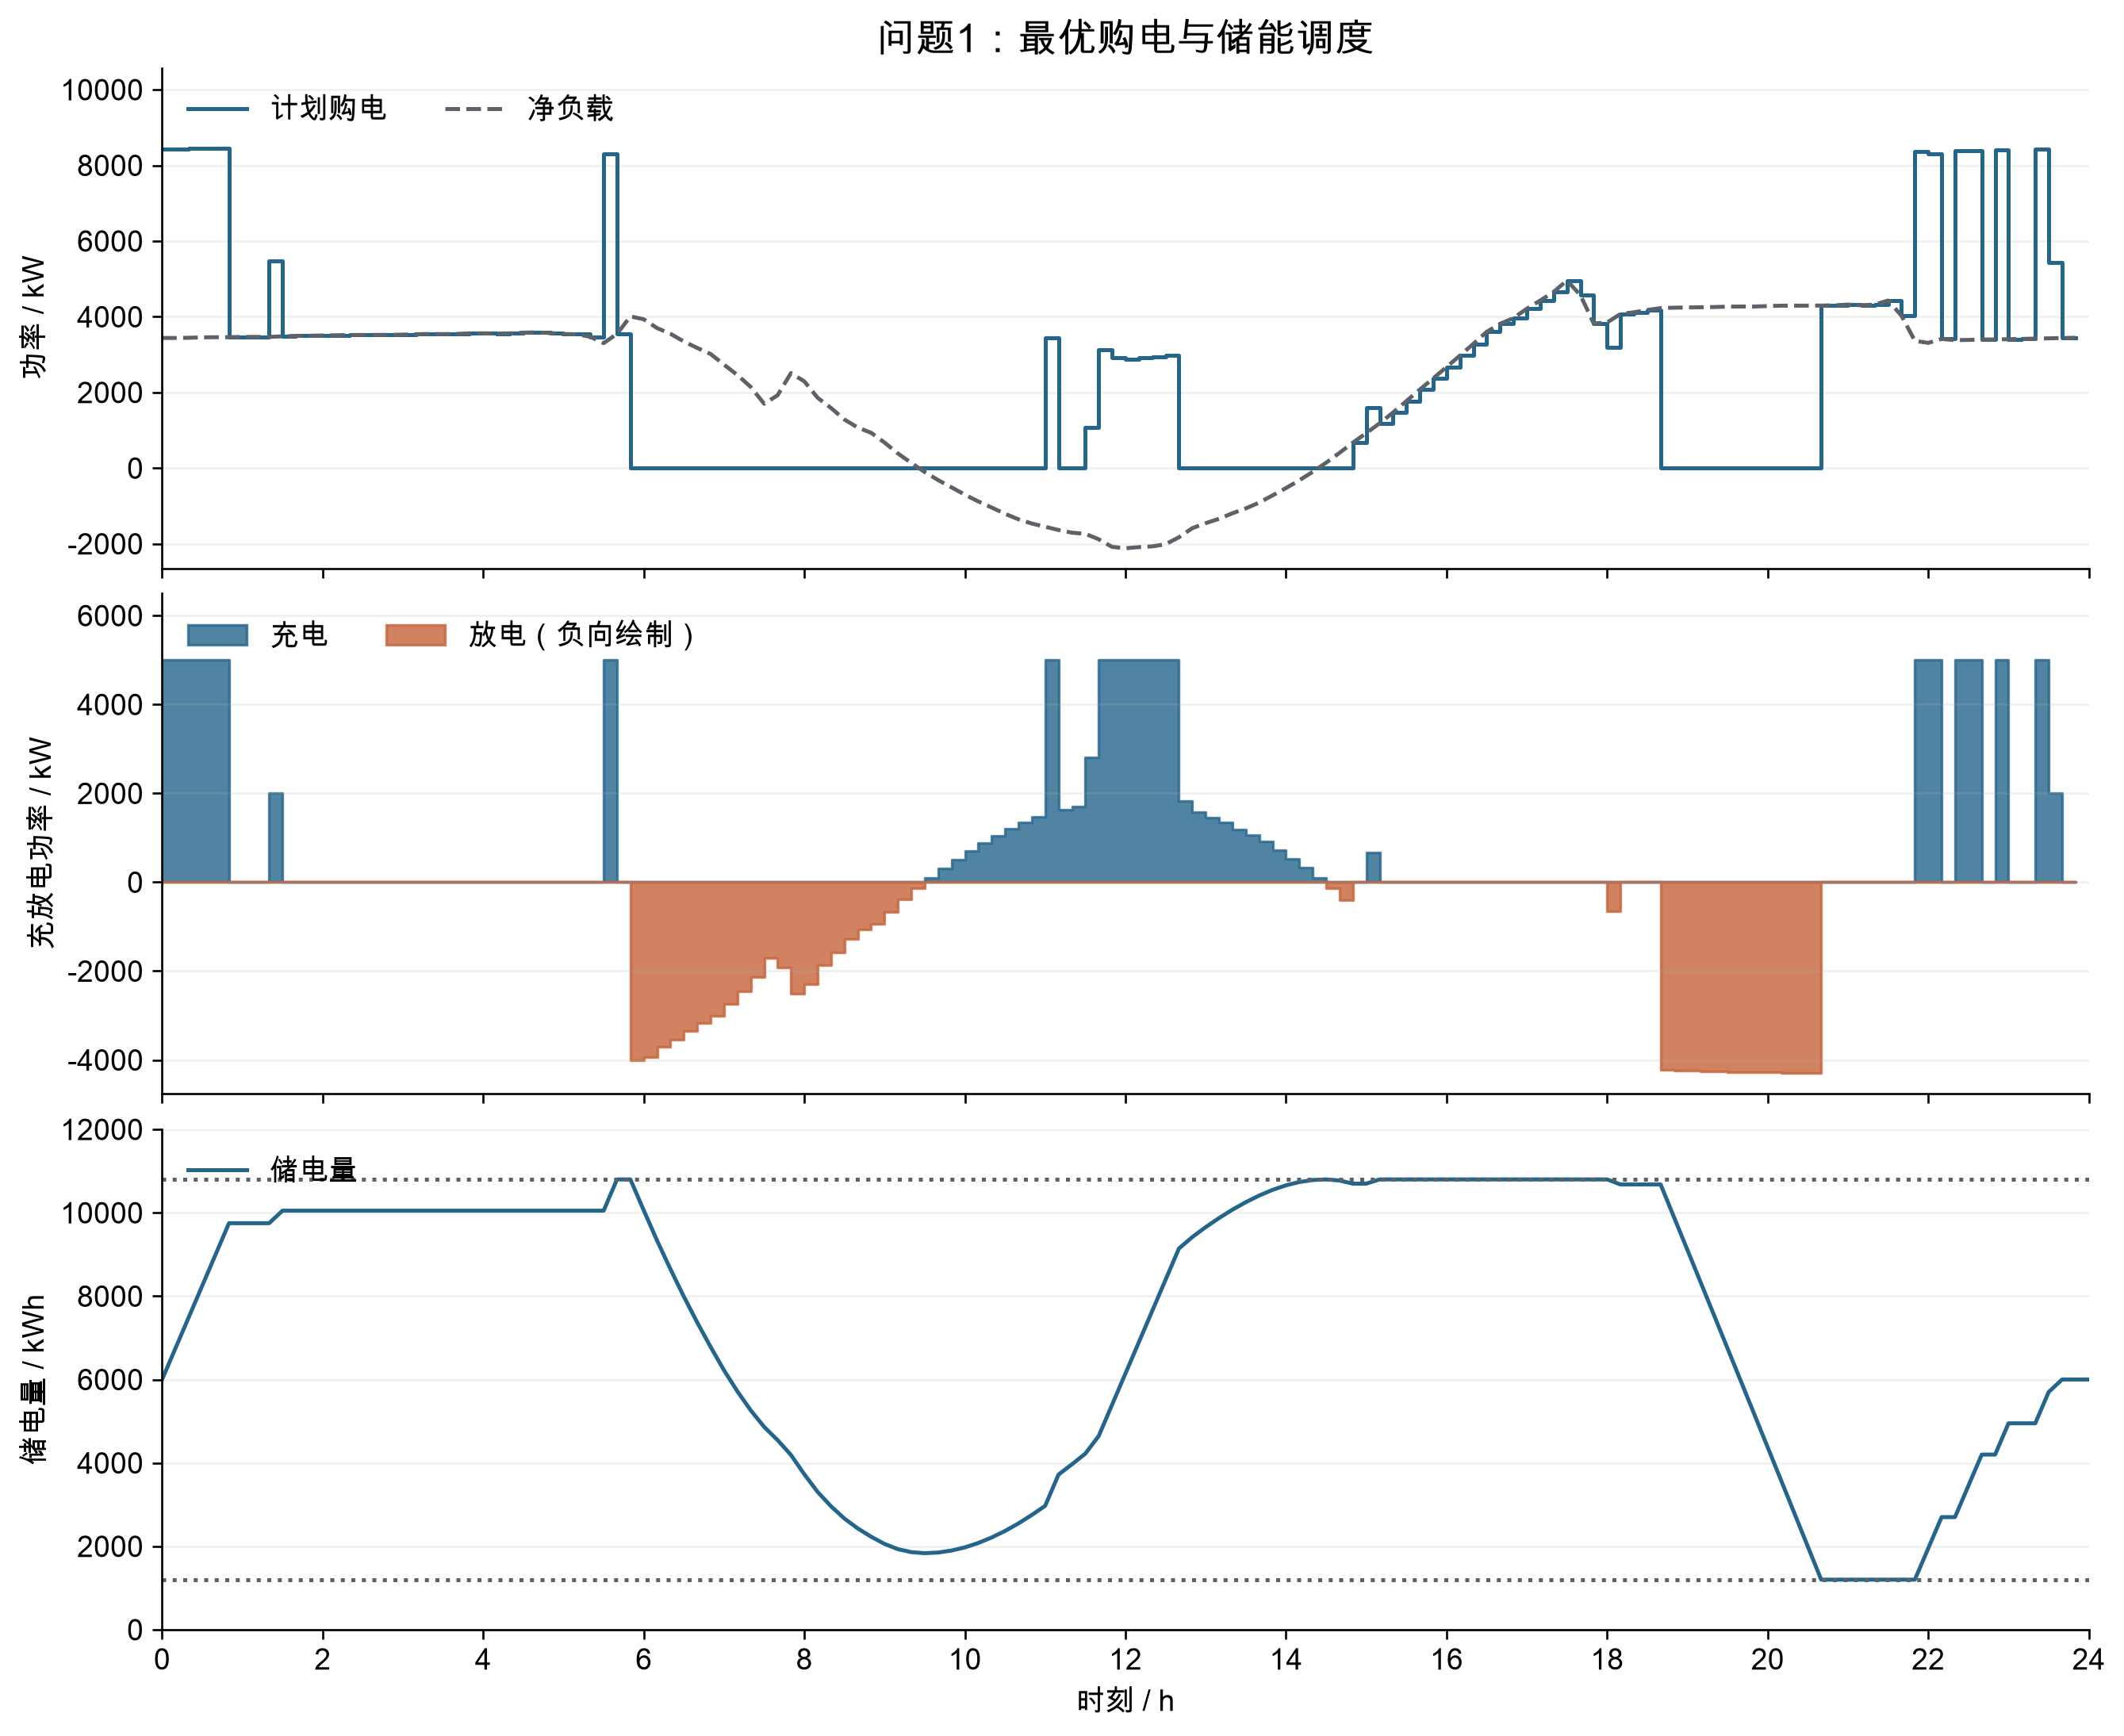
\includegraphics[width=\linewidth,height=9.0cm,keepaspectratio]{figures/q1.png}
\caption{代表日购电与储能调度（提供结果）}\label{fig:q1}
\end{figure}

\section{问题二：历史预测下的固定合同}
\subsection{预测与经验风险裕度}
历史同时段预测为过去$W$日观测的指数加权平均，较近日期权重较高。对负载、光伏或电价变量$Y$，令$n=\min(d,W)$，其预测为
\begin{equation}
\widehat Y^{\rm EW}_{d,t}=\frac{\sum_{k=1}^{n}\exp[-\alpha(k-1)]Y_{d-k,t}}{\sum_{k=1}^{n}\exp[-\alpha(k-1)]}.
\end{equation}
上式适用于$d\ge1$；无历史的初日采用附件一曲线作为先验。负载预测在存在同星期历史样本时，与此前最多四个同星期几的均值各按一半融合：
\begin{equation}
\widehat L_{d,t}=\tfrac12\widehat L^{\rm EW}_{d,t}+\tfrac12\operatorname{mean}\{L_{d-7k,t}:1\le k\le4,\ d-7k\ge0\}.
\end{equation}
若$d<7$，同星期历史样本集合为空，则直接使用指数加权预测，不计算空集合均值。

预测评价采用训练区间与正式评价区间分离的原则，误差指标的定义参照预测学教材\cite{forecast}。在1月15日至31日按均方根误差选择预测参数，负载采用14日窗口、0.1衰减率并保留星期因素，历史光伏采用7日窗口、0.1衰减率。二月以后固定这些参数，只随日期推进更新历史样本。

记净负载预测误差为$e_{j,s}=L_{j,s}-PV_{j,s}-\widehat L_{j,s}+\widehat{PV}_{j,s}$。以两小时为误差分块$B(t)$，构造
\begin{align}
M_{d,t}&=\max\{0,Q_q(\{e_{j,s}:\max(0,d-21)\le j<d,\ s\in B(t)\})\},\\
N^{\rm safe}_{d,t}&=\widehat L_{d,t}-\widehat{PV}_{d,t}+M_{d,t}.
\end{align}
安全分位数$q$是管理参数，其值不能直接解释为全天无紧急购电的概率。使用已完成日期的误差，避免当天未来样本进入风险估计。

\subsection{固定合同规划与参数}
每天零时，以此前历史数据构成信息集。用$\widetilde C_t,\widetilde D_t,\widetilde R_t,\widetilde E_t$表示规划变量，求解
\begin{align}
\min\quad &\sum_{t=0}^{143}\widehat p_tG_t^0\Delta t,\\
\text{s.t.}\quad&G_t^0+\widetilde D_t=N_t^{\rm safe}+\widetilde C_t+\widetilde R_t,\\
&\widetilde E_{t+1}=\widetilde E_t+\eta\widetilde C_t\Delta t-\widetilde D_t\Delta t/\eta,\\
&\widetilde E_0=E_{d,0},\quad \widetilde E_{144}=E^{\rm tar},
\end{align}
同时施加统一的非负、储电范围、功率及充放电互斥约束。规划不安排紧急购电。问题二电价已知，故$\widehat p_t=p_t$；问题四则用预测电价。
本问$q=0.70$、$E^{\rm tar}=3600$ kWh。末端目标只约束预测规划，实际日末库存由实时执行决定，并传递给下一日。

一月热启动采用预先固定的7日窗口、0.3衰减率、0.8安全分位数与6,000 kWh末端目标，从1月1日6,000 kWh运行至2月1日10,800 kWh。参数搜索以一月费用减去0.5元/kWh的库存变化估值为准，采用有限候选坐标搜索。该库存估值只用于参数比较，不进入实际费用。提供代码中的动态规划执行器仅为校准候选，本次主结果使用贪心纠偏。

\subsection{运行结果}
实际费用按$J_2=\sum_t p_t(G_t^0+5X_t)\Delta t$计算。334日实际费用为15,176,691.87元，紧急购电量为286,749.92 kWh，12月31日末储电量为3,590.82 kWh。图\ref{fig:q2}中，计划购电无需逐点贴合净负载预测，两者之间的差额还要由储能吸收或补足。合同一经固定，多购但未利用的电量仍需付费；少购超过储能可补范围时，则按五倍电价应急补足。因此，增加安全裕度的代价必须与减少的应急费用一起比较。


\begin{figure}[htbp]\centering
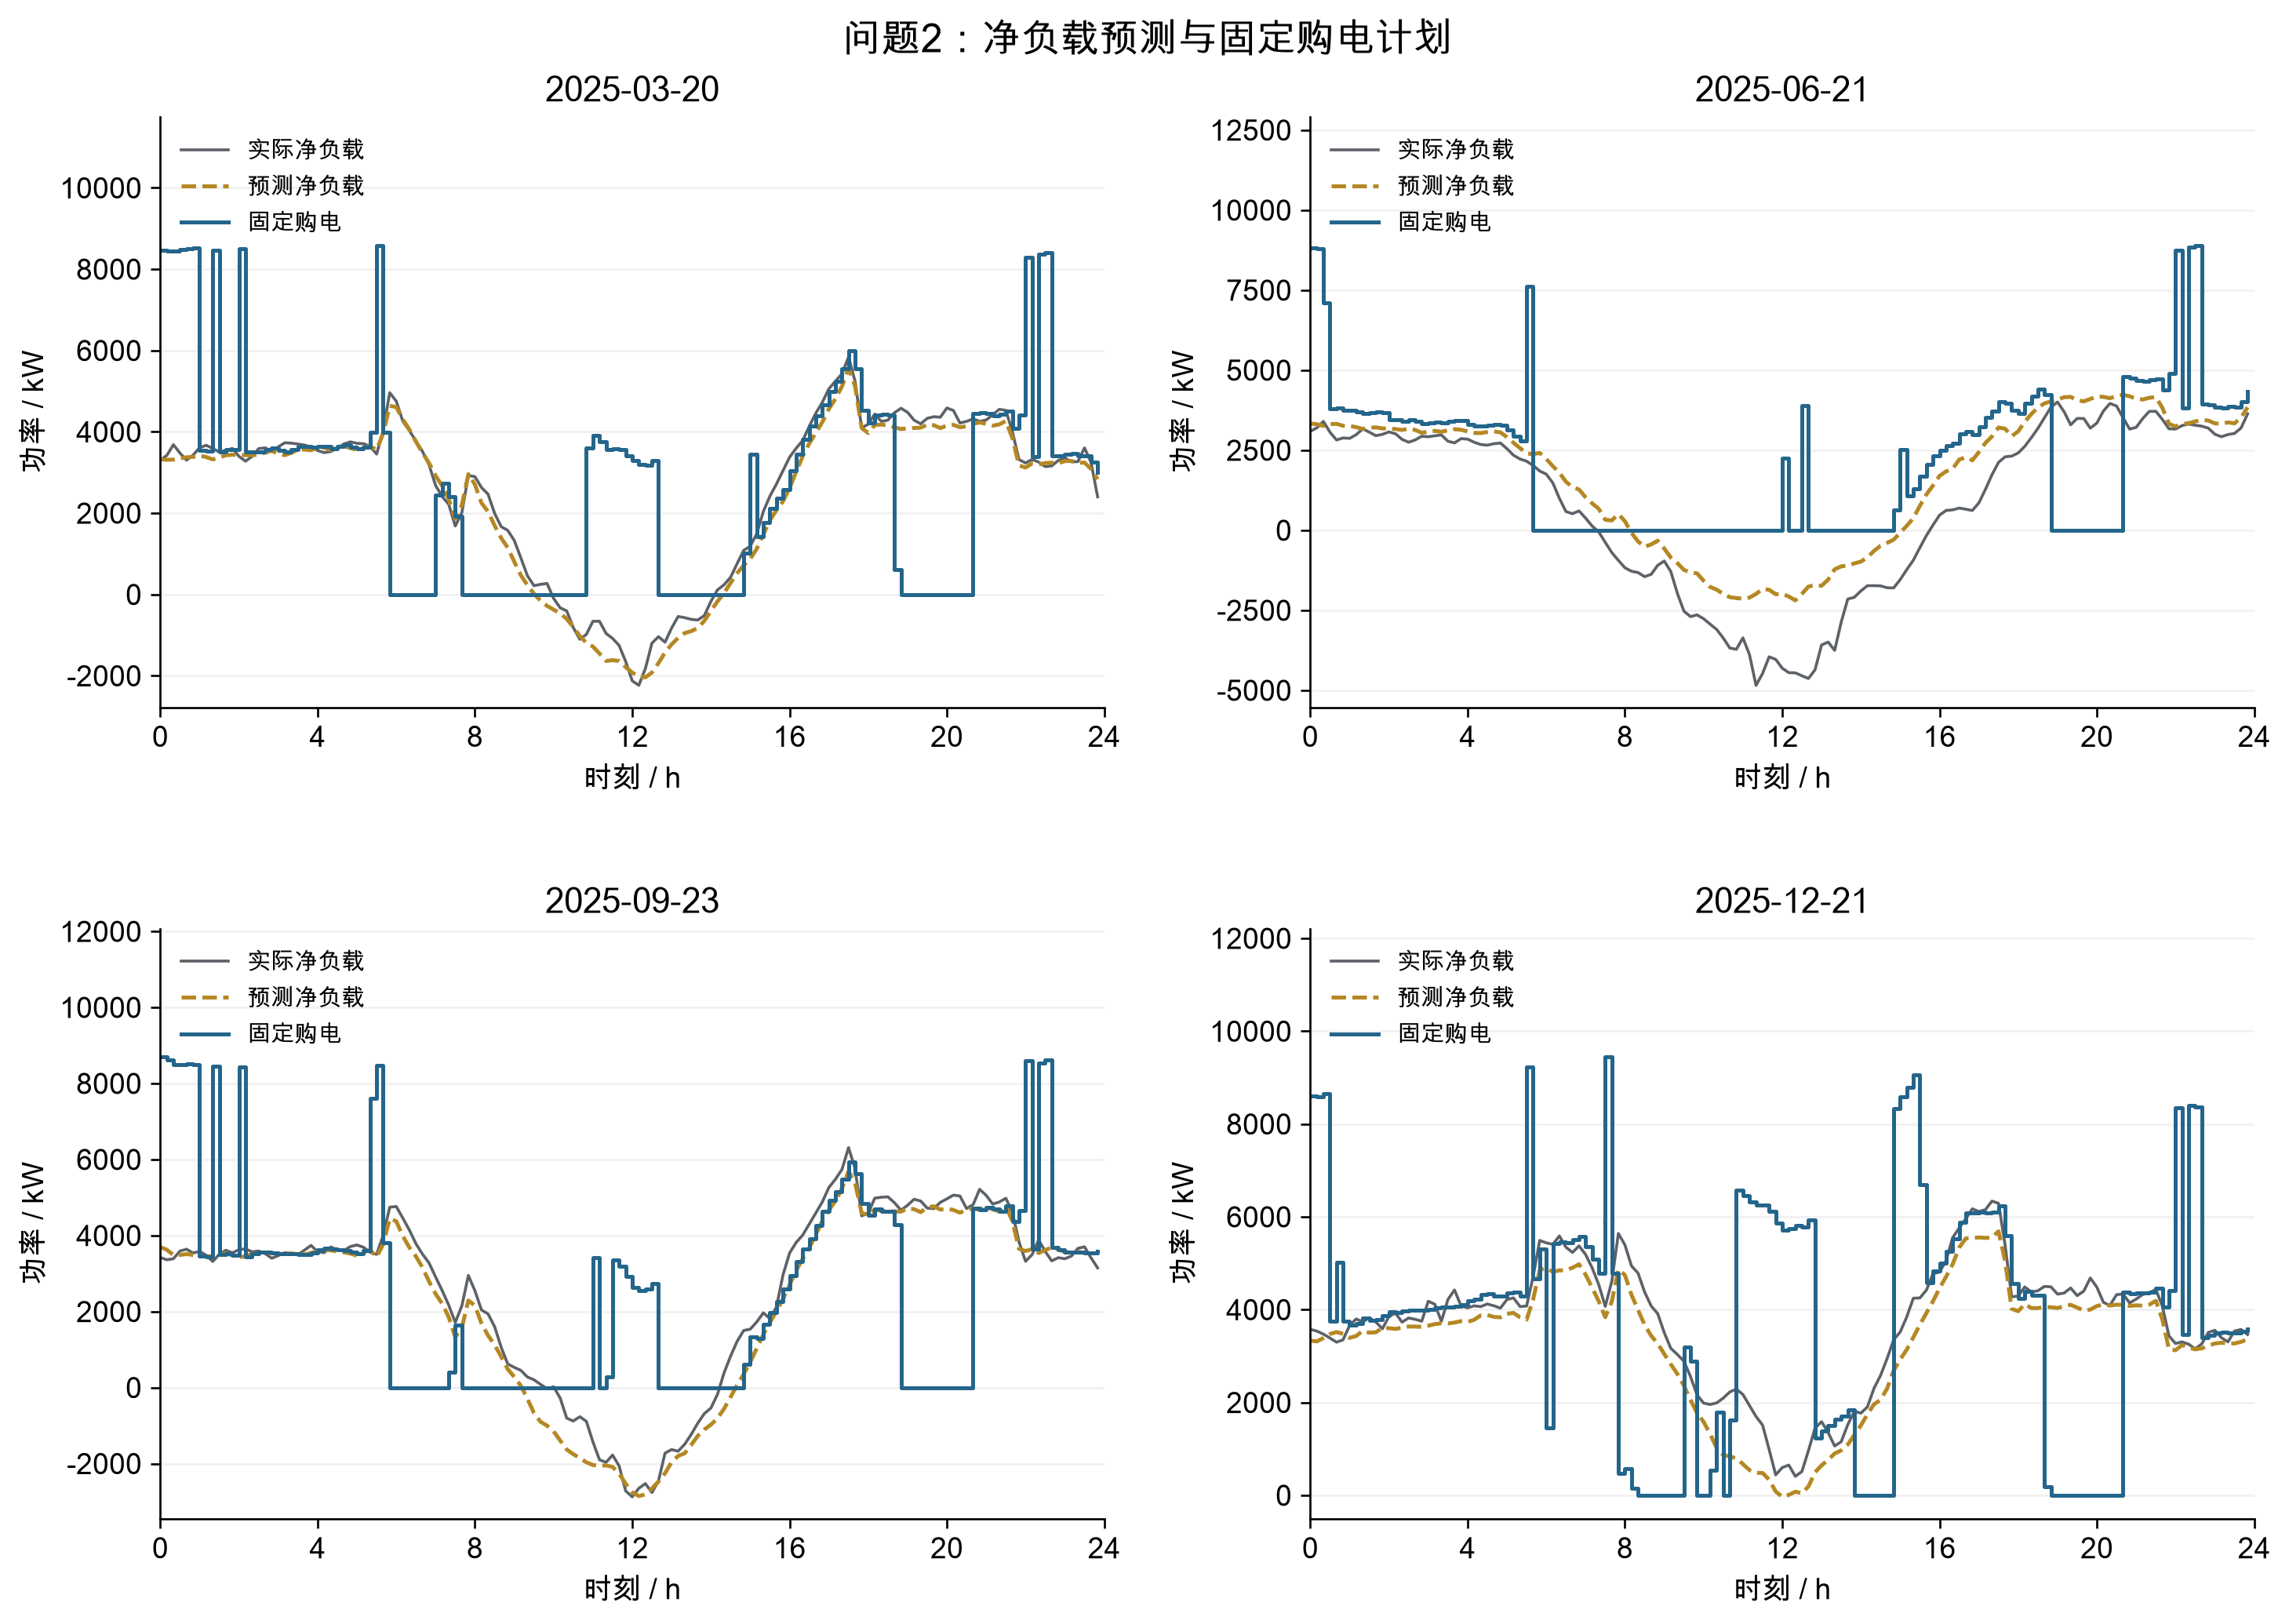
\includegraphics[width=\linewidth,height=9.0cm,keepaspectratio]{figures/q2.png}
\caption{指定日期净负载预测与固定购电计划}\label{fig:q2}
\end{figure}

\section{问题三：光伏更新与滚动合同}
\subsection{发布预报融合}
在0、6、12、18时仅使用当时已经发布的光伏预报。用发布时刻已观测光伏作锚点，将整点预测线性插值到十分钟网格；按过去21个完整日、相同发布时刻及相同两小时目标区间计算预测平均偏差$\bar b$，再融合历史预测：
\begin{equation}
\widehat{PV}^{\rm corr}=\max\{0,\widehat{PV}^{\rm raw}-\bar b\},\qquad
\widehat{PV}=w_h\widehat{PV}^{\rm corr}+(1-w_h)\widehat{PV}^{\rm hist}.
\end{equation}
一月选出的四个发布时间权重依次为0.25、0.75、0.75、0。18时权重仅针对当天剩余时段，不能据此判断其未来24小时预报整体无效。本问安全分位数为0.65，末端目标为3,600 kWh。每个发布时刻的安全裕度仍取此前21个完整日，但误差统一定义为实际净负载减预测净负载，即$e_{j,s\mid h}=L_{j,s}-PV_{j,s}-\widehat L_{j,s}+\widehat{PV}_{j,s\mid h}$。正误差表示低估供电需求，安全裕度据此取非负分位数。

\subsection{剩余合同优化与费用}
文献\cite{mpc}将混合整数规划与模型预测控制用于微网管理。本文借鉴随状态和预测更新剩余计划的思路，每六小时重新决策合同，两个更新时刻之间仍按实际缺口执行储能纠偏。

在6、12、18时，以实际储电量作为新初值，保持已经执行的时段不变，重新优化当日剩余合同。令$u_t=(G_t^0-a_t)^+$、$v_t=(a_t-G_t^0)^+$，其中$(x)^+=\max(x,0)$，则
\begin{equation}
J_3=\sum_t p_t\left[G_t^0-0.5u_t+1.5v_t+5X_t\right]\Delta t.
\end{equation}
例如原计划100 kWh、最终80 kWh、价格1元/kWh时，合同结算为$100-20+10=90$元。若取消后原款不退，则取消部分净系数应改为$+0.5$，本模型全部滚动费用均需重新计算。

设当前发布时刻对应第$k$个十分钟时段，剩余规划区间为$\mathcal T_k=\{k,\ldots,143\}$。以当前实际库存$E_{d,k}$为初值，沿用上述规划物理约束，但将合同变量改为$a_t$，并允许规划应急量$\widetilde X_t$：
\begin{align}
a_t+\widetilde D_t+\widetilde X_t&=N^{\rm safe}_{t\mid k}+\widetilde C_t+\widetilde R_t,\\
a_t+u_t-v_t&=G_t^0,\qquad u_t,v_t\ge0.
\end{align}
剩余规划以$\sum_{t\in\mathcal T_k}\widehat p_{t\mid k}(G_t^0-0.5u_t+1.5v_t+5\widetilde X_t)\Delta t$最小为目标，并保持规划末端目标。价格为正，同一时段同时增加$u_t,v_t$会提高费用，因此最优解自然避免无意义的同时退订与增购。规划应急量只用于评价剩余合同，并非已发生的紧急购电；实际$X_t$仍由真实缺口决定。

滚动规划允许预测紧急购电，以比较增购与应急补足的代价。对保留合同和候选合同，采用同一预测及执行器计算剩余费用，记候选执行评估得到的期末库存为$\widetilde E^{\rm eval}_{144}$，再加入$0.5\max\{E^{\rm tar}-\widetilde E^{\rm eval}_{144},0\}$的末端不足估值；仅当候选估计费用更低且超过数值容差时接受调整。这里的评估库存由同一安全净负载情景和贪心执行器推演得到，不是实际日末观测，也不必等于规划末端目标。实际结算不包含这项估值。

\subsection{结果与更新价值}
本问334日实际费用为14,145,706.54元，紧急购电为96,886.54 kWh，期末储电为3,536.55 kWh。图\ref{fig:q3}给出指定日期原计划与最终合同的差异。相较第二问费用减少1,030,985.32元；由于光伏信息、合同调整权及安全分位数同时改变，此差额是两套完整策略的比较，不能单独归因于某一模块。
\begin{figure}[htbp]\centering
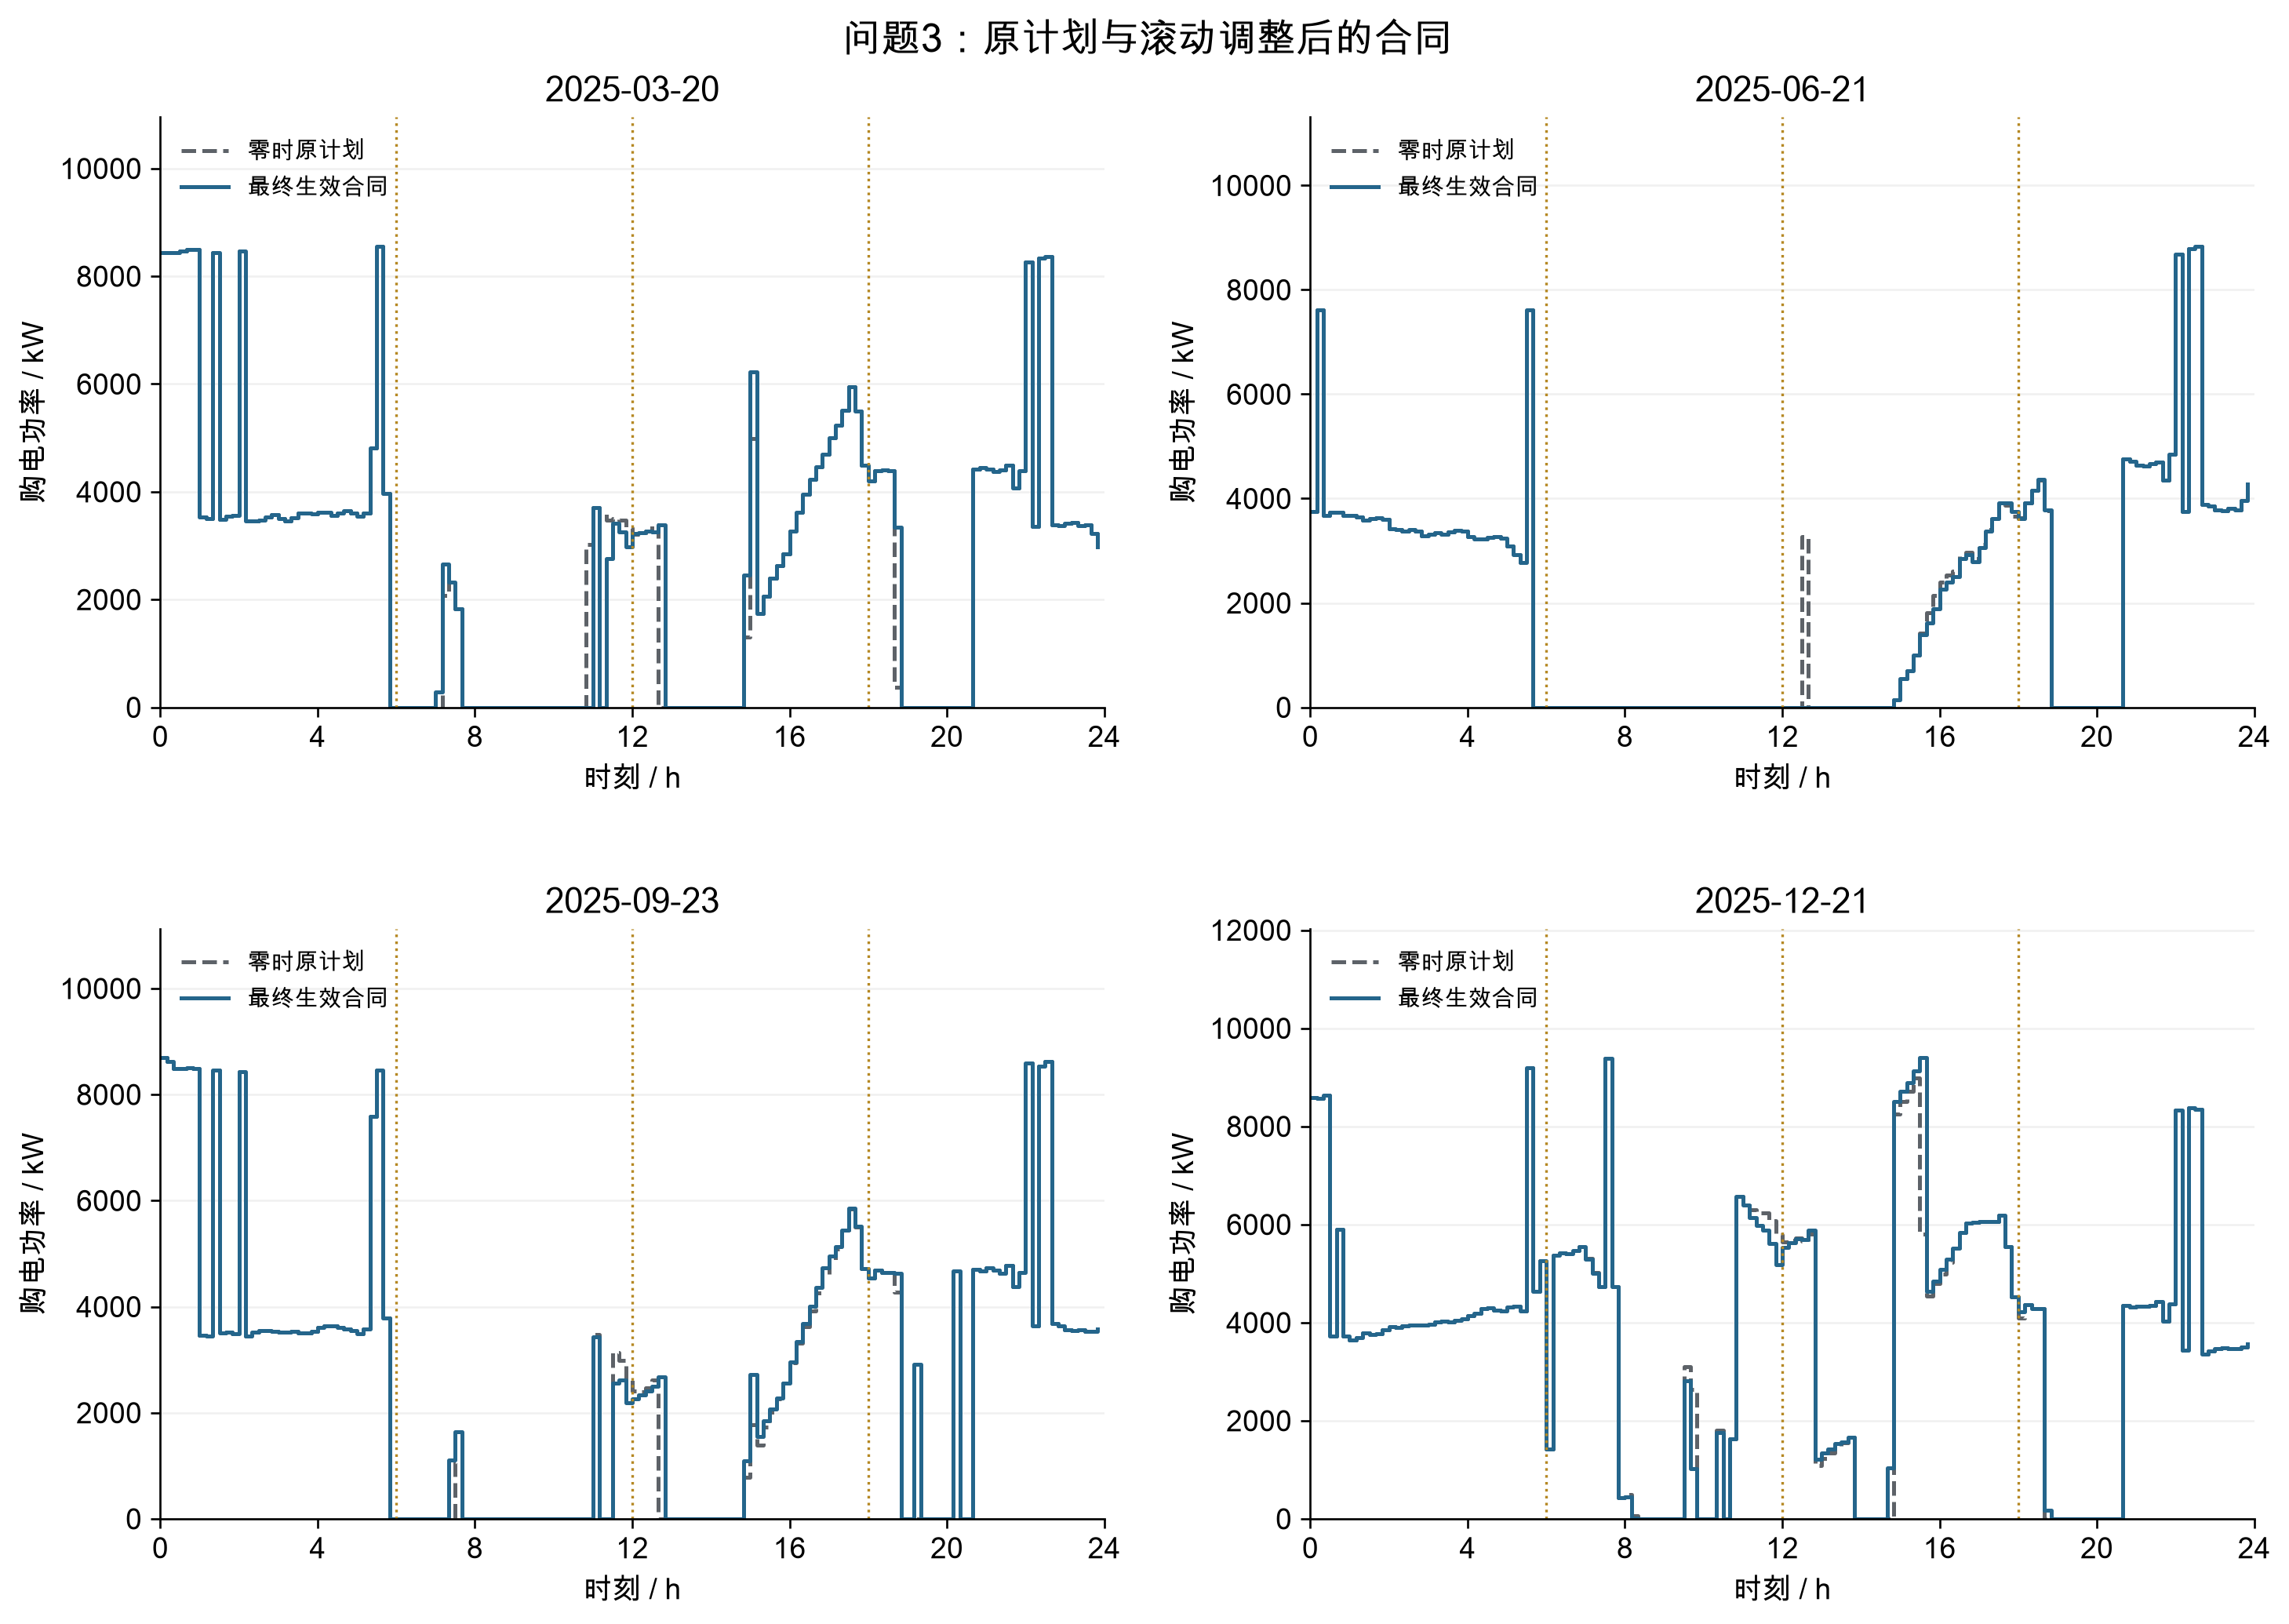
\includegraphics[width=\linewidth,height=9.0cm,keepaspectratio]{figures/q3.png}
\caption{指定日期的零时合同与最终调整合同}\label{fig:q3}
\end{figure}

为判断是否引入其他时刻预报，首先在相同交付区间07:00--18:00比较预报误差，其次比较仅零时合同与滚动执行的经济结果。误差统计由逐点预测误差重算，各组覆盖334日、每天66个共同目标时段，见表\ref{tab:2}。RMSE定义为误差平方均值的平方根，MAE为绝对误差均值，两者单位均为kW。


\par\addvspace{5pt}\noindent\begin{minipage}{\linewidth}\centering
\small
\papertable{共同目标区间光伏预报误差}\par\vspace{4pt}
\begin{tabular}{lrrr}
\toprule
预报来源 & RMSE/kW & MAE/kW & 样本数 \\
\midrule
前日18时原始 & 776.56 & 564.83 & 22044 \\
当日0时原始 & 562.05 & 409.20 & 22044 \\
当日6时原始 & 343.51 & 246.14 & 22044 \\
当日0时融合 & 381.96 & 276.63 & 22044 \\
当日6时融合 & 301.71 & 217.11 & 22044 \\
\bottomrule
\end{tabular}
\end{minipage}\par\addvspace{5pt}


\par\addvspace{5pt}\noindent\begin{minipage}{\linewidth}\centering
\small
\papertable{相同模型下的更新策略对照（提供的对照结果）}\par\vspace{4pt}
\begin{tabular}{lrrr}
\toprule
策略 & 实际费用/元 & 紧急电量/kWh & 接受更新次数 \\
\midrule
仅零时合同 & 15,358,890.57 & 348,985.29 & 0 \\
每次重优化 & 14,145,706.54 & 96,886.55 & 1002 \\
价值触发 & 14,145,706.54 & 96,886.54 & 991 \\
\bottomrule
\end{tabular}
\end{minipage}\par\addvspace{5pt}

表\ref{tab:2}中，原始预报的RMSE从零时的562.05 kW降至6时的343.51 kW，6时融合预报进一步降至301.71 kW；MAE也呈同样变化。在所比较的07:00--18:00交付区间内，临近交付获得的预报更准确。其余交付区间未纳入这组共同样本，不能直接沿用这一判断。

表\ref{tab:3}固定预测与参数配置，仅改变更新规则。价值触发相对仅零时合同节省1,213,184.03元，同时减少紧急购电；与每次重优化相比，则仅少接受11次更新，费用差不足0.01元。这组结果支持使用日内更新，但尚未显示价值触发有额外的节费作用。预报误差下降能否转化为费用下降，还取决于可用储电量和合同调整价格。




\section{问题四：未知未来电价下的调度}
\subsection{价格预测与信息边界}
图\ref{fig:q4price}展示价格预测与实际值的偏差。附件四作为实际交付电价记录。零时价格预测使用此前14日同一时段观测的指数加权平均，衰减率为0.1，参数只在一月选择。滚动情形在发布时刻$h\in\{6,12,18\}$，根据过去六小时已经发生的价格偏差修正未来预测：
\begin{equation}
\widehat p_{d,t\mid h}=\max\left\{0.001,\widehat p_{d,t\mid0}+0.5\operatorname{mean}_{s\in[h-6,h)}(p_{d,s}-\widehat p_{d,s\mid0})\right\}.
\end{equation}
式中集合以小时描述，实际计算采用对应的36个十分钟时段。固定合同不能日内调整且采用贪心执行，故上述价格修正不改变其动作。实际结算始终使用$p_{d,t}$，不是预测价。
\begin{figure}[htbp]\centering
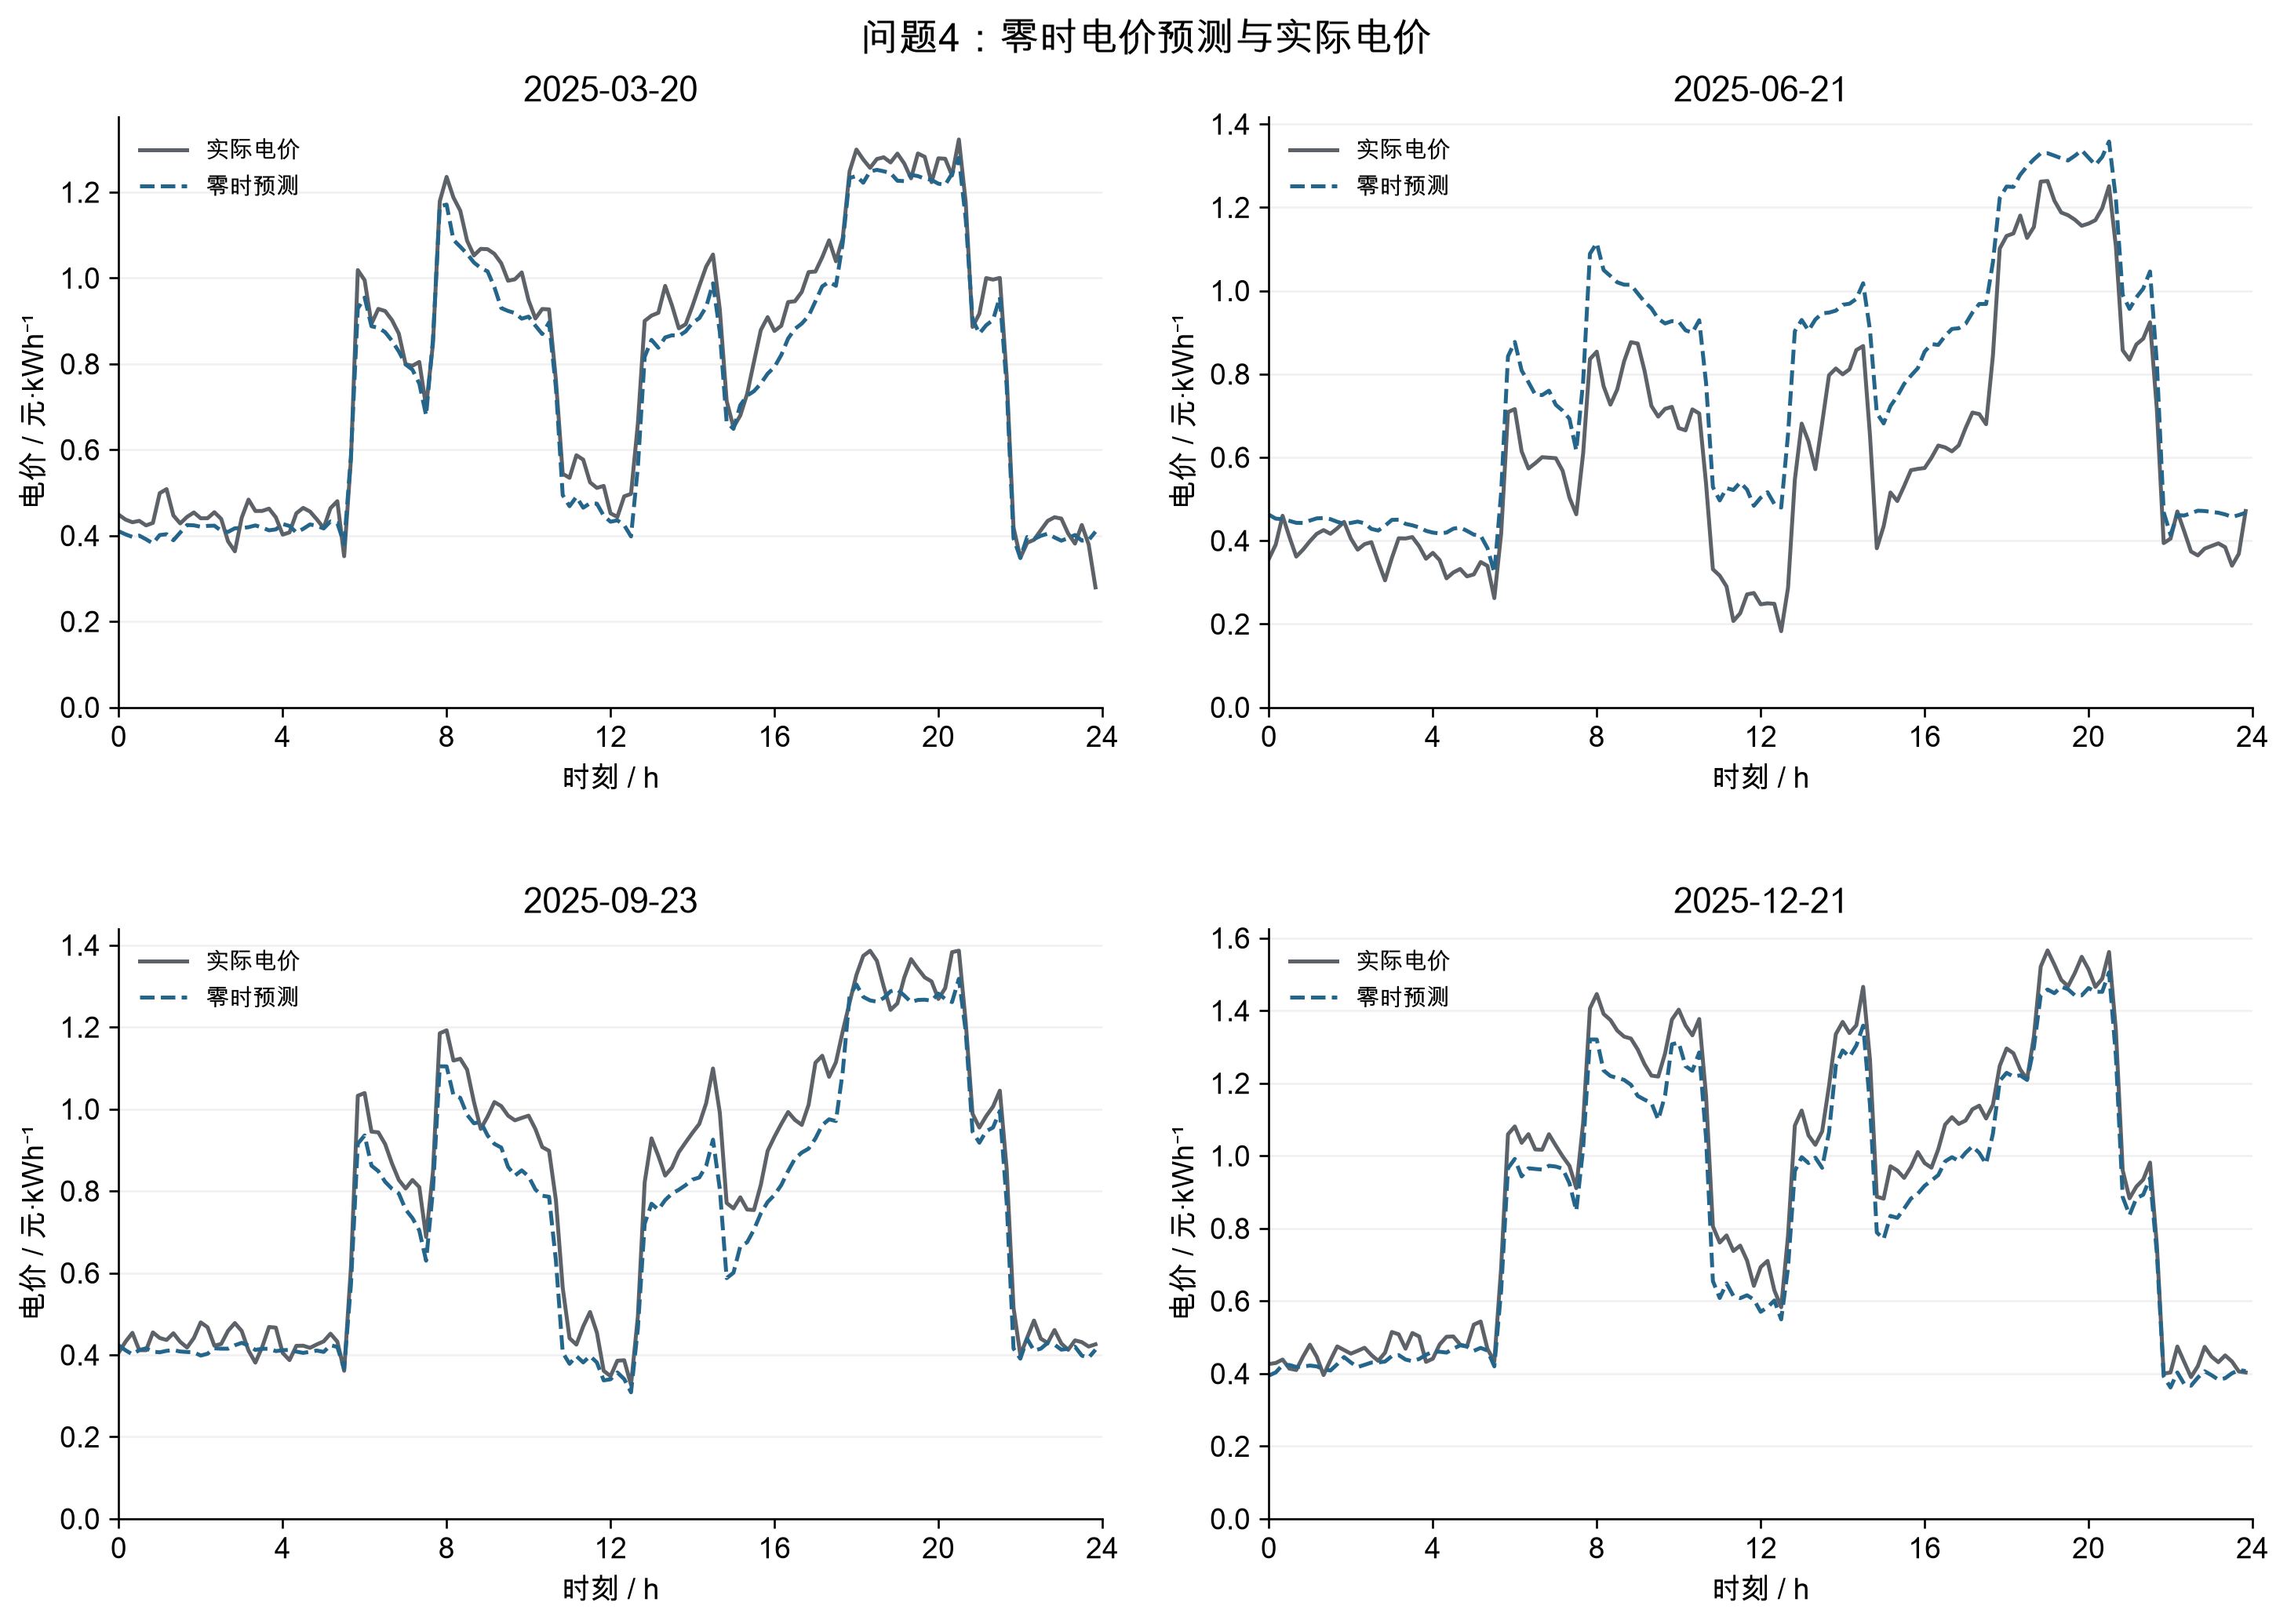
\includegraphics[width=\linewidth,height=9.0cm,keepaspectratio]{figures/q4price.png}
\caption{指定日期的零时价格预测与实际电价}\label{fig:q4price}
\end{figure}

\subsection{参数与结果比较}
固定合同安全分位数0.70，滚动合同0.65，两者规划末端目标均为6,000 kWh。除价格信息和末端目标外，分别沿用第二、三问的模型结构。一月仍执行共同的固定电价热启动策略，至2月1日取得10,800 kWh库存；这是为正式期比较设置的共同历史运行条件，并非按附件四价格重新优化一月的结果。问题四的波动价格调度从正式期开始评价。各情形正式统计见表\ref{tab:4}。


\par\addvspace{5pt}\noindent\begin{minipage}{\linewidth}\centering
\small
\papertable{2月至12月各情形运行结果}\par\vspace{4pt}
\begin{tabular}{lrrr}
\toprule
情形 & 总费用/元 & 紧急电量/kWh & 期末储电/kWh \\
\midrule
问题二 & 15,176,691.87 & 286,749.92 & 3,590.82 \\
问题三 & 14,145,706.54 & 96,886.54 & 3,536.55 \\
问题四：固定合同 & 15,834,890.34 & 292,350.50 & 5,980.54 \\
问题四：滚动合同 & 14,799,117.00 & 101,962.18 & 5,936.52 \\
\bottomrule
\end{tabular}
\end{minipage}\par\addvspace{5pt}

波动电价下，滚动合同较固定合同节省1,035,773.34元，降幅6.54\%，紧急购电量由292,350.50 kWh降至101,962.18 kWh。两者期末储电分别为5,980.54与5,936.52 kWh，费用比较未作期末库存价值调整。部分指定日滚动费用可能高于固定合同，全年汇总改善不代表逐日占优。





图\ref{fig:monthly}将累计结果分解到各月，同时呈现费用与紧急购电量，便于区分经济性和应急需求。两项指标分别计算，不用费用下降替代供电风险评价。
\begin{figure}[!htbp]\centering

\includegraphics[width=\linewidth]{figures/monthly.pdf}
\caption{波动电价下固定与滚动合同的月度比较}\label{fig:monthly}
\end{figure}
\section{结果核验、敏感性与模型评价}
\subsection{逐时一致性核验}
对192,528条逐时记录检查功率平衡、储电递推、跨时段库存衔接、费用分项、储电及功率上下限和充放电互斥，均满足$10^{-5}$的相应单位绝对误差容差。负载、光伏和结算电价逐项回查原始附件，未发现错位。五份结果工作簿中的购电与储能数值也与逐时记录一致。

进一步在独立目录中使用Python 3.12.13、SciPy 1.18.1重新执行四问主求解入口，五种情形均运行成功。重算结果与原记录各数值列的最大绝对差不超过$3.00\times10^{-6}$，主要费用保留两位小数后相同。这说明既定参数下的主运行可复现，并不证明题意解释唯一正确，也不构成未知未来条件下的全局最优证明。

该复现使用既定管理参数；预测参数与融合权重按代码重新准备，但未重新执行安全分位数、末端目标等管理参数的完整搜索。

\subsection{风险裕度与效率敏感性}
表\ref{tab:5}与表\ref{tab:6}的单因素分析固定其他最终参数，安全分位数比较使用1月15日至31日，效率比较使用2月至12月。两者统计区间不同，费用不能直接横向比较；敏感性实验本次仅核对提供文件，未独立重跑。


\par\addvspace{5pt}\noindent\begin{minipage}{\linewidth}\centering
\small
\papertable{问题三安全分位数单因素分析（一月校准区间）}\par\vspace{4pt}
\begin{tabular}{lrrr}
\toprule
分位数 & 费用/元 & 紧急电量/kWh & 库存调整评分/元 \\
\midrule
0.60 & 920,541.05 & 2,887.12 & 919,897.09 \\
0.65 & 919,693.92 & 1,580.13 & 918,974.32 \\
0.70 & 924,025.95 & 653.25 & 923,246.75 \\
0.75 & 935,873.43 & 199.36 & 935,032.19 \\
0.80 & 956,151.22 & 108.31 & 955,241.23 \\
0.85 & 984,710.78 & 42.66 & 983,717.93 \\
0.90 & 1,022,943.82 & 22.91 & 1,021,845.26 \\
\bottomrule
\end{tabular}
\end{minipage}\par\addvspace{5pt}

表\ref{tab:5}中，0.65的库存调整评分最低。分位数由0.65提高到0.70后，紧急购电量从1,580.13 kWh降至653.25 kWh，总费用却从919,693.92元升至924,025.95元。更保守的计划减少了应急需求，但新增合同支出超过了相应节省。该比较来自一月校准区间，用于解释参数取值，不代表二月至十二月重新调参的结果。


\par\addvspace{5pt}\noindent\begin{minipage}{\linewidth}\centering
\small
\papertable{问题三单侧效率敏感性（2月至12月）}\par\vspace{4pt}
\begin{tabular}{lrrr}
\toprule
单侧效率 & 费用/元 & 紧急电量/kWh & 期末储电/kWh \\
\midrule
0.85 & 14,612,065.38 & 85,907.68 & 3,527.02 \\
0.90 & 14,145,706.54 & 96,886.54 & 3,536.55 \\
0.95 & 13,678,086.84 & 100,128.47 & 3,545.38 \\
\bottomrule
\end{tabular}
\end{minipage}\par\addvspace{5pt}

表\ref{tab:6}中，单侧效率从0.85升至0.95时，总费用从14,612,065.38元降至13,678,086.84元，紧急购电量却从85,907.68 kWh升至100,128.47 kWh。费用与应急电量没有同向变化，说明效率变化后需分别检查合同、储能及应急购电的运行结果。这组实验固定了管理参数，不能解释为每种效率下重新寻优所得的费用曲线。

\subsection{退订结算口径的重新优化对照}
若退订后原计划款不退，费用应写为
\begin{equation}
J^{\rm nr}=\sum_t p_t[G_t^0+0.5u_t+1.5v_t+5X_t]\Delta t.
\end{equation}
该变化同时进入剩余合同优化、候选更新评价及实际结算。固定原有预测参数、安全分位数、末端目标和共同初始库存，重新运行2月至12月全部时段，得到下列结果。这是给定参数下的策略重算，不是重新校准全部参数后的最优结果。
\par\addvspace{5pt}\noindent\begin{minipage}{\linewidth}\centering\small
\textbf{退订不退款的补充对照}\par\vspace{4pt}
\begin{tabular}{lrr}\toprule
情形 & 实际费用/元 & 紧急购电/kWh\\\midrule
问题三 & 14,179,773.58 & 95,334.47\\
问题四滚动 & 14,829,340.66 & 100,457.80\\\bottomrule
\end{tabular}\end{minipage}\par\addvspace{5pt}
相应固定合同费用分别为15,176,691.87元和15,834,890.34元。比较仅用于检验两套完整策略在另一结算口径下的累计表现，不能单独识别滚动信息的因果收益。前述价值触发与每次重优化相差不足0.01元的判断仅对应退款口径，不延伸到此补充实验。五份主结果Excel仍对应正文主口径，补充逐时数据单独提供。

\subsection{适用性与局限}
合同电量、实际储能动作和结算费用可以逐时对应，便于检查预测偏差最终由哪一项承担。应用范围仍受三个条件限制：经验分位数未显式描述误差在连续时段内的相关性；贪心执行未充分衡量后续库存价值；设备寿命、网络约束和紧急购电容量尚未纳入。因而本文费用结果用于比较给定条件下的运行策略，尚不足以直接估算实际项目的投资收益或供电可靠性。

\section{结论}
已知代表日曲线时，储能通过跨时段充放电降低购电费用；曲线未知时，合同还需承担预测误差。固定合同用历史误差裕度提前留出余量，滚动合同则利用新预报调整未交付电量，实际偏差最终由储能和紧急购电共同消化。

在主退款口径下，两组电价条件的滚动策略累计费用均低于相应固定策略，但逐日费用并非始终更低。更新规则对照进一步表明，主要收益来自使用日内更新；价值触发少接受11次更新，却没有可辨认的额外节费。这些判断以本文信息条件、参数及退订结算口径为前提，不能外推为任意条件下的最优策略。

\section{指定日期与时段结果}
本节依次给出各问指定结果，表\ref{tab:7}起的购电表和储能表可与相应模型结果对应阅读。以下表格直接由逐时结果汇总，电量单位均为kWh，费用单位均为元。购电表按题目六个指定时段排布，充放电表按四小时区间双栏排布。滚动情形分别列出零时计划与最终合同；最终合同表所列合同结算费包含调整结算，不含紧急费。累计电量使用未四舍五入的逐时值计算，表内分项保留两位小数，可能出现0.01的显示尾差。

\subsection{问题一代表日}


\par\addvspace{5pt}\noindent\begin{minipage}{\linewidth}\centering
\small
\papertable{计划购电：代表日}\par\vspace{4pt}
\begin{tabular}{lrlrlr}
\toprule
时间段 & 电量 & 时间段 & 电量 & 时间段 & 电量 \\
\midrule
10:00-10:10 & 0.00 & 12:00-12:10 & 480.41 & 14:00-14:10 & 0.00 \\
16:00-16:10 & 445.43 & 18:00-18:10 & 531.89 & 20:00-20:10 & 0.00 \\
全天购电 & 59,482.70 & 合同购电费 & 35,126.95 &  &  \\
\bottomrule
\end{tabular}
\end{minipage}\par\addvspace{5pt}


\par\addvspace{5pt}\noindent\begin{minipage}{\linewidth}\centering
\small
\papertable{储能运行：代表日}\par\vspace{4pt}
\begin{tabular}{lrrlrr}
\toprule
时间段 & 充电量 & 放电量 & 时间段 & 充电量 & 放电量 \\
\midrule
00:00--04:00 & 4,500.00 & 0.00 & 04:00--08:00 & 833.33 & 6,365.84 \\
08:00--12:00 & 4,787.96 & 1,703.00 & 12:00--16:00 & 5,286.04 & 91.10 \\
16:00--20:00 & 0.00 & 5,780.13 & 20:00--24:00 & 5,333.33 & 2,859.87 \\
0:00储电 & 6,000.00 &  & 24:00储电 & 6,000.00 &  \\
\bottomrule
\end{tabular}
\end{minipage}\par\addvspace{5pt}


\subsection{问题二}

\Needspace{7\baselineskip}\subsubsection{2025-03-20}


\par\addvspace{5pt}\noindent\begin{minipage}{\linewidth}\centering
\small
\papertable{计划购电：2025-03-20}\par\vspace{4pt}
\begin{tabular}{lrlrlr}
\toprule
时间段 & 电量 & 时间段 & 电量 & 时间段 & 电量 \\
\midrule
10:00-10:10 & 0.00 & 12:00-12:10 & 548.55 & 14:00-14:10 & 0.00 \\
16:00-16:10 & 507.45 & 18:00-18:10 & 703.19 & 20:00-20:10 & 0.00 \\
全天购电 & 66,145.41 & 合同购电费 & 40,046.63 &  &  \\
\bottomrule
\end{tabular}
\end{minipage}\par\addvspace{5pt}


\par\addvspace{5pt}\noindent\begin{minipage}{\linewidth}\centering
\small
\papertable{储能运行：2025-03-20}\par\vspace{4pt}
\begin{tabular}{lrrlrr}
\toprule
时间段 & 充电量 & 放电量 & 时间段 & 充电量 & 放电量 \\
\midrule
00:00--04:00 & 6,680.68 & 150.50 & 04:00--08:00 & 1,076.98 & 5,679.14 \\
08:00--12:00 & 5,888.90 & 2,777.38 & 12:00--16:00 & 4,641.35 & 507.07 \\
16:00--20:00 & 228.35 & 5,859.65 & 20:00--24:00 & 3,032.16 & 2,604.79 \\
0:00储电 & 4,002.78 &  & 24:00储电 & 3,864.66 &  \\
\bottomrule
\end{tabular}
\end{minipage}\par\addvspace{5pt}

该日紧急购电费为2,673.80元，实际总费用为42,720.43元。

\Needspace{7\baselineskip}\subsubsection{2025-06-21}


\par\addvspace{5pt}\noindent\begin{minipage}{\linewidth}\centering
\small
\papertable{计划购电：2025-06-21}\par\vspace{4pt}
\begin{tabular}{lrlrlr}
\toprule
时间段 & 电量 & 时间段 & 电量 & 时间段 & 电量 \\
\midrule
10:00-10:10 & 0.00 & 12:00-12:10 & 377.11 & 14:00-14:10 & 0.00 \\
16:00-16:10 & 416.90 & 18:00-18:10 & 609.59 & 20:00-20:10 & 0.00 \\
全天购电 & 52,015.33 & 合同购电费 & 32,050.51 &  &  \\
\bottomrule
\end{tabular}
\end{minipage}\par\addvspace{5pt}


\par\addvspace{5pt}\noindent\begin{minipage}{\linewidth}\centering
\small
\papertable{储能运行：2025-06-21}\par\vspace{4pt}
\begin{tabular}{lrrlrr}
\toprule
时间段 & 充电量 & 放电量 & 时间段 & 充电量 & 放电量 \\
\midrule
00:00--04:00 & 3,058.83 & 0.00 & 04:00--08:00 & 344.45 & 1,719.95 \\
08:00--12:00 & 1,778.95 & 0.00 & 12:00--16:00 & 0.00 & 0.00 \\
16:00--20:00 & 0.00 & 4,169.91 & 20:00--24:00 & 5,350.52 & 2,485.90 \\
0:00储电 & 8,047.05 &  & 24:00储电 & 8,220.13 &  \\
\bottomrule
\end{tabular}
\end{minipage}\par\addvspace{5pt}

该日紧急购电费为0.00元，实际总费用为32,050.51元。



\Needspace{7\baselineskip}\subsubsection{2025-09-23}


\par\addvspace{5pt}\noindent\begin{minipage}{\linewidth}\centering
\small
\papertable{计划购电：2025-09-23}\par\vspace{4pt}
\begin{tabular}{lrlrlr}
\toprule
时间段 & 电量 & 时间段 & 电量 & 时间段 & 电量 \\
\midrule
10:00-10:10 & 0.00 & 12:00-12:10 & 440.02 & 14:00-14:10 & 0.00 \\
16:00-16:10 & 491.54 & 18:00-18:10 & 756.38 & 20:00-20:10 & 0.00 \\
全天购电 & 63,880.49 & 合同购电费 & 39,160.62 &  &  \\
\bottomrule
\end{tabular}
\end{minipage}\par\addvspace{5pt}


\par\addvspace{5pt}\noindent\begin{minipage}{\linewidth}\centering
\small
\papertable{储能运行：2025-09-23}\par\vspace{4pt}
\begin{tabular}{lrrlrr}
\toprule
时间段 & 充电量 & 放电量 & 时间段 & 充电量 & 放电量 \\
\midrule
00:00--04:00 & 6,625.98 & 156.78 & 04:00--08:00 & 1,532.39 & 6,962.96 \\
08:00--12:00 & 4,607.71 & 1,524.37 & 12:00--16:00 & 5,476.64 & 769.76 \\
16:00--20:00 & 54.31 & 6,519.26 & 20:00--24:00 & 2,835.28 & 962.76 \\
0:00储电 & 3,458.27 &  & 24:00储电 & 3,704.12 &  \\
\bottomrule
\end{tabular}
\end{minipage}\par\addvspace{5pt}

该日紧急购电费为19,425.27元，实际总费用为58,585.89元。

\Needspace{7\baselineskip}\subsubsection{2025-12-21}


\par\addvspace{5pt}\noindent\begin{minipage}{\linewidth}\centering
\small
\papertable{计划购电：2025-12-21}\par\vspace{4pt}
\begin{tabular}{lrlrlr}
\toprule
时间段 & 电量 & 时间段 & 电量 & 时间段 & 电量 \\
\midrule
10:00-10:10 & 0.00 & 12:00-12:10 & 951.84 & 14:00-14:10 & 0.00 \\
16:00-16:10 & 833.63 & 18:00-18:10 & 707.35 & 20:00-20:10 & 0.00 \\
全天购电 & 91,144.09 & 合同购电费 & 59,031.51 &  &  \\
\bottomrule
\end{tabular}
\end{minipage}\par\addvspace{5pt}


\par\addvspace{5pt}\noindent\begin{minipage}{\linewidth}\centering
\small
\papertable{储能运行：2025-12-21}\par\vspace{4pt}
\begin{tabular}{lrrlrr}
\toprule
时间段 & 充电量 & 放电量 & 时间段 & 充电量 & 放电量 \\
\midrule
00:00--04:00 & 3,198.34 & 150.34 & 04:00--08:00 & 1,420.53 & 1,558.20 \\
08:00--12:00 & 5,481.67 & 7,491.52 & 12:00--16:00 & 7,619.71 & 2,287.26 \\
16:00--20:00 & 86.42 & 6,024.16 & 20:00--24:00 & 2,855.99 & 2,723.70 \\
0:00储电 & 7,615.47 &  & 24:00储电 & 3,728.33 &  \\
\bottomrule
\end{tabular}
\end{minipage}\par\addvspace{5pt}

该日紧急购电费为1,255.96元，实际总费用为60,287.47元。

\par\addvspace{6pt}\noindent\begin{minipage}{\linewidth}\centering\scriptsize\papertable{四个指定日期的紧急购电}\par\vspace{4pt}
\begin{tabular}{lrlrlrlr}\toprule

\multicolumn{2}{c}{03-20} & \multicolumn{2}{c}{06-21} & \multicolumn{2}{c}{09-23} & \multicolumn{2}{c}{12-21} \\

时段 & 电量 & 时段 & 电量 & 时段 & 电量 & 时段 & 电量 \\ \midrule

20:30--20:40 & 383.29 & 无 & 0.00 & 08:40--09:50 & 372.25 & 07:50--08:00 & 28.05 \\
 &  &  &  & 20:10--21:50 & 2,673.86 & 20:30--20:40 & 156.69 \\

\bottomrule\end{tabular}\end{minipage}\par\addvspace{6pt}


\subsection{问题三}

\Needspace{7\baselineskip}\subsubsection{2025-03-20}


\par\addvspace{5pt}\noindent\begin{minipage}{\linewidth}\centering
\small
\papertable{零时计划：2025-03-20}\par\vspace{4pt}
\begin{tabular}{lrlrlr}
\toprule
时间段 & 电量 & 时间段 & 电量 & 时间段 & 电量 \\
\midrule
10:00-10:10 & 0.00 & 12:00-12:10 & 536.11 & 14:00-14:10 & 0.00 \\
16:00-16:10 & 544.91 & 18:00-18:10 & 700.21 & 20:00-20:10 & 0.00 \\
全天购电 & 65,877.29 & 原计划费 & 39,844.35 &  &  \\
\bottomrule
\end{tabular}
\end{minipage}\par\addvspace{5pt}


\par\addvspace{5pt}\noindent\begin{minipage}{\linewidth}\centering
\small
\papertable{最终合同：2025-03-20}\par\vspace{4pt}
\begin{tabular}{lrlrlr}
\toprule
时间段 & 电量 & 时间段 & 电量 & 时间段 & 电量 \\
\midrule
10:00-10:10 & 0.00 & 12:00-12:10 & 537.28 & 14:00-14:10 & 0.00 \\
16:00-16:10 & 544.91 & 18:00-18:10 & 700.21 & 20:00-20:10 & 0.00 \\
全天购电 & 66,128.46 & 合同结算费 & 41,522.61 &  &  \\
\bottomrule
\end{tabular}
\end{minipage}\par\addvspace{5pt}


\par\addvspace{5pt}\noindent\begin{minipage}{\linewidth}\centering
\small
\papertable{储能运行：2025-03-20}\par\vspace{4pt}
\begin{tabular}{lrrlrr}
\toprule
时间段 & 充电量 & 放电量 & 时间段 & 充电量 & 放电量 \\
\midrule
00:00--04:00 & 6,650.94 & 215.89 & 04:00--08:00 & 1,158.14 & 6,059.20 \\
08:00--12:00 & 4,350.14 & 2,456.81 & 12:00--16:00 & 5,927.37 & 305.57 \\
16:00--20:00 & 240.86 & 5,327.17 & 20:00--24:00 & 2,969.41 & 2,965.83 \\
0:00储电 & 3,873.94 &  & 24:00储电 & 3,785.03 &  \\
\bottomrule
\end{tabular}
\end{minipage}\par\addvspace{5pt}

该日紧急购电费为1,867.19元，实际总费用为43,389.79元。



\Needspace{7\baselineskip}\subsubsection{2025-06-21}


\par\addvspace{5pt}\noindent\begin{minipage}{\linewidth}\centering
\small
\papertable{零时计划：2025-06-21}\par\vspace{4pt}
\begin{tabular}{lrlrlr}
\toprule
时间段 & 电量 & 时间段 & 电量 & 时间段 & 电量 \\
\midrule
10:00-10:10 & 0.00 & 12:00-12:10 & 0.00 & 14:00-14:10 & 0.00 \\
16:00-16:10 & 400.47 & 18:00-18:10 & 605.41 & 20:00-20:10 & 0.00 \\
全天购电 & 48,585.61 & 原计划费 & 30,189.70 &  &  \\
\bottomrule
\end{tabular}
\end{minipage}\par\addvspace{5pt}


\par\addvspace{5pt}\noindent\begin{minipage}{\linewidth}\centering
\small
\papertable{最终合同：2025-06-21}\par\vspace{4pt}
\begin{tabular}{lrlrlr}
\toprule
时间段 & 电量 & 时间段 & 电量 & 时间段 & 电量 \\
\midrule
10:00-10:10 & 0.00 & 12:00-12:10 & 0.00 & 14:00-14:10 & 0.00 \\
16:00-16:10 & 376.22 & 18:00-18:10 & 603.40 & 20:00-20:10 & 0.00 \\
全天购电 & 47,871.87 & 合同结算费 & 30,039.49 &  &  \\
\bottomrule
\end{tabular}
\end{minipage}\par\addvspace{5pt}


\par\addvspace{5pt}\noindent\begin{minipage}{\linewidth}\centering
\small
\papertable{储能运行：2025-06-21}\par\vspace{4pt}
\begin{tabular}{lrrlrr}
\toprule
时间段 & 充电量 & 放电量 & 时间段 & 充电量 & 放电量 \\
\midrule
00:00--04:00 & 2,871.14 & 0.00 & 04:00--08:00 & 721.84 & 1,719.95 \\
08:00--12:00 & 1,778.95 & 0.00 & 12:00--16:00 & 0.00 & 0.00 \\
16:00--20:00 & 0.00 & 4,169.91 & 20:00--24:00 & 5,209.42 & 2,485.90 \\
0:00储电 & 7,876.33 &  & 24:00储电 & 8,093.14 &  \\
\bottomrule
\end{tabular}
\end{minipage}\par\addvspace{5pt}

该日紧急购电费为0.00元，实际总费用为30,039.49元。



\Needspace{7\baselineskip}\subsubsection{2025-09-23}


\par\addvspace{5pt}\noindent\begin{minipage}{\linewidth}\centering
\small
\papertable{零时计划：2025-09-23}\par\vspace{4pt}
\begin{tabular}{lrlrlr}
\toprule
时间段 & 电量 & 时间段 & 电量 & 时间段 & 电量 \\
\midrule
10:00-10:10 & 0.00 & 12:00-12:10 & 402.26 & 14:00-14:10 & 0.00 \\
16:00-16:10 & 491.63 & 18:00-18:10 & 756.39 & 20:00-20:10 & 0.00 \\
全天购电 & 63,455.07 & 原计划费 & 38,893.95 &  &  \\
\bottomrule
\end{tabular}
\end{minipage}\par\addvspace{5pt}


\par\addvspace{5pt}\noindent\begin{minipage}{\linewidth}\centering
\small
\papertable{最终合同：2025-09-23}\par\vspace{4pt}
\begin{tabular}{lrlrlr}
\toprule
时间段 & 电量 & 时间段 & 电量 & 时间段 & 电量 \\
\midrule
10:00-10:10 & 0.00 & 12:00-12:10 & 378.12 & 14:00-14:10 & 0.00 \\
16:00-16:10 & 493.94 & 18:00-18:10 & 756.39 & 20:00-20:10 & 0.00 \\
全天购电 & 65,570.28 & 合同结算费 & 42,589.43 &  &  \\
\bottomrule
\end{tabular}
\end{minipage}\par\addvspace{5pt}


\par\addvspace{5pt}\noindent\begin{minipage}{\linewidth}\centering
\small
\papertable{储能运行：2025-09-23}\par\vspace{4pt}
\begin{tabular}{lrrlrr}
\toprule
时间段 & 充电量 & 放电量 & 时间段 & 充电量 & 放电量 \\
\midrule
00:00--04:00 & 6,625.98 & 156.78 & 04:00--08:00 & 1,519.79 & 6,868.59 \\
08:00--12:00 & 4,381.94 & 1,608.54 & 12:00--16:00 & 6,103.97 & 586.92 \\
16:00--20:00 & 34.48 & 5,949.92 & 20:00--24:00 & 2,835.28 & 2,024.15 \\
0:00储电 & 3,458.27 &  & 24:00储电 & 3,704.12 &  \\
\bottomrule
\end{tabular}
\end{minipage}\par\addvspace{5pt}

该日紧急购电费为6,553.59元，实际总费用为49,143.01元。



\Needspace{7\baselineskip}\subsubsection{2025-12-21}


\par\addvspace{5pt}\noindent\begin{minipage}{\linewidth}\centering
\small
\papertable{零时计划：2025-12-21}\par\vspace{4pt}
\begin{tabular}{lrlrlr}
\toprule
时间段 & 电量 & 时间段 & 电量 & 时间段 & 电量 \\
\midrule
10:00-10:10 & 0.00 & 12:00-12:10 & 940.71 & 14:00-14:10 & 0.00 \\
16:00-16:10 & 831.90 & 18:00-18:10 & 680.92 & 20:00-20:10 & 0.00 \\
全天购电 & 90,133.16 & 原计划费 & 58,207.18 &  &  \\
\bottomrule
\end{tabular}
\end{minipage}\par\addvspace{5pt}


\par\addvspace{5pt}\noindent\begin{minipage}{\linewidth}\centering
\small
\papertable{最终合同：2025-12-21}\par\vspace{4pt}
\begin{tabular}{lrlrlr}
\toprule
时间段 & 电量 & 时间段 & 电量 & 时间段 & 电量 \\
\midrule
10:00-10:10 & 0.00 & 12:00-12:10 & 921.88 & 14:00-14:10 & 0.00 \\
16:00-16:10 & 847.30 & 18:00-18:10 & 702.81 & 20:00-20:10 & 0.00 \\
全天购电 & 90,526.40 & 合同结算费 & 59,273.05 &  &  \\
\bottomrule
\end{tabular}
\end{minipage}\par\addvspace{5pt}


\par\addvspace{5pt}\noindent\begin{minipage}{\linewidth}\centering
\small
\papertable{储能运行：2025-12-21}\par\vspace{4pt}
\begin{tabular}{lrrlrr}
\toprule
时间段 & 充电量 & 放电量 & 时间段 & 充电量 & 放电量 \\
\midrule
00:00--04:00 & 3,285.81 & 189.10 & 04:00--08:00 & 1,570.97 & 1,590.12 \\
08:00--12:00 & 5,120.85 & 7,806.67 & 12:00--16:00 & 8,171.97 & 2,127.18 \\
16:00--20:00 & 76.94 & 6,074.51 & 20:00--24:00 & 2,807.50 & 2,688.11 \\
0:00储电 & 7,479.87 &  & 24:00储电 & 3,659.75 &  \\
\bottomrule
\end{tabular}
\end{minipage}\par\addvspace{5pt}

该日紧急购电费为2,056.45元，实际总费用为61,329.50元。

\par\addvspace{6pt}\noindent\begin{minipage}{\linewidth}\centering\scriptsize\papertable{四个指定日期的紧急购电}\par\vspace{4pt}
\begin{tabular}{lrlrlrlr}\toprule

\multicolumn{2}{c}{03-20} & \multicolumn{2}{c}{06-21} & \multicolumn{2}{c}{09-23} & \multicolumn{2}{c}{12-21} \\

时段 & 电量 & 时段 & 电量 & 时段 & 电量 & 时段 & 电量 \\ \midrule

09:10--10:00 & 320.57 & 无 & 0.00 & 08:50--09:50 & 288.08 & 07:50--08:00 & 35.17 \\
20:30--20:40 & 43.07 &  &  & 20:20--21:50 & 833.91 & 10:40--10:50 & 88.69 \\
 &  &  &  &  &  & 20:30--20:40 & 214.71 \\

\bottomrule\end{tabular}\end{minipage}\par\addvspace{6pt}


\subsection{问题四：固定合同}

\Needspace{7\baselineskip}\subsubsection{2025-03-20}


\par\addvspace{5pt}\noindent\begin{minipage}{\linewidth}\centering
\small
\papertable{计划购电：2025-03-20}\par\vspace{4pt}
\begin{tabular}{lrlrlr}
\toprule
时间段 & 电量 & 时间段 & 电量 & 时间段 & 电量 \\
\midrule
10:00-10:10 & 0.00 & 12:00-12:10 & 548.55 & 14:00-14:10 & 0.00 \\
16:00-16:10 & 507.45 & 18:00-18:10 & 0.00 & 20:00-20:10 & 733.12 \\
全天购电 & 66,082.80 & 合同购电费 & 41,055.26 &  &  \\
\bottomrule
\end{tabular}
\end{minipage}\par\addvspace{5pt}


\par\addvspace{5pt}\noindent\begin{minipage}{\linewidth}\centering
\small
\papertable{储能运行：2025-03-20}\par\vspace{4pt}
\begin{tabular}{lrrlrr}
\toprule
时间段 & 充电量 & 放电量 & 时间段 & 充电量 & 放电量 \\
\midrule
00:00--04:00 & 4,056.29 & 150.50 & 04:00--08:00 & 1,024.51 & 5,679.14 \\
08:00--12:00 & 5,888.90 & 2,777.38 & 12:00--16:00 & 4,641.35 & 507.07 \\
16:00--20:00 & 112.51 & 7,213.01 & 20:00--24:00 & 5,675.62 & 1,169.11 \\
0:00储电 & 6,459.13 &  & 24:00储电 & 6,278.16 &  \\
\bottomrule
\end{tabular}
\end{minipage}\par\addvspace{5pt}

该日紧急购电费为2,108.61元，实际总费用为43,163.87元。

\Needspace{7\baselineskip}\subsubsection{2025-06-21}


\par\addvspace{5pt}\noindent\begin{minipage}{\linewidth}\centering
\small
\papertable{计划购电：2025-06-21}\par\vspace{4pt}
\begin{tabular}{lrlrlr}
\toprule
时间段 & 电量 & 时间段 & 电量 & 时间段 & 电量 \\
\midrule
10:00-10:10 & 0.00 & 12:00-12:10 & 0.00 & 14:00-14:10 & 0.00 \\
16:00-16:10 & 416.90 & 18:00-18:10 & 609.59 & 20:00-20:10 & 0.00 \\
全天购电 & 52,041.96 & 合同购电费 & 27,576.59 &  &  \\
\bottomrule
\end{tabular}
\end{minipage}\par\addvspace{5pt}


\par\addvspace{5pt}\noindent\begin{minipage}{\linewidth}\centering
\small
\papertable{储能运行：2025-06-21}\par\vspace{4pt}
\begin{tabular}{lrrlrr}
\toprule
时间段 & 充电量 & 放电量 & 时间段 & 充电量 & 放电量 \\
\midrule
00:00--04:00 & 682.54 & 190.97 & 04:00--08:00 & 344.45 & 1,382.92 \\
08:00--12:00 & 1,362.85 & 0.00 & 12:00--16:00 & 0.00 & 0.00 \\
16:00--20:00 & 0.00 & 4,755.36 & 20:00--24:00 & 7,696.91 & 1,865.03 \\
0:00储电 & 10,397.90 &  & 24:00储电 & 10,371.22 &  \\
\bottomrule
\end{tabular}
\end{minipage}\par\addvspace{5pt}

该日紧急购电费为0.00元，实际总费用为27,576.59元。



\Needspace{7\baselineskip}\subsubsection{2025-09-23}


\par\addvspace{5pt}\noindent\begin{minipage}{\linewidth}\centering
\small
\papertable{计划购电：2025-09-23}\par\vspace{4pt}
\begin{tabular}{lrlrlr}
\toprule
时间段 & 电量 & 时间段 & 电量 & 时间段 & 电量 \\
\midrule
10:00-10:10 & 0.00 & 12:00-12:10 & 440.02 & 14:00-14:10 & 0.00 \\
16:00-16:10 & 491.54 & 18:00-18:10 & 0.00 & 20:00-20:10 & 0.00 \\
全天购电 & 63,885.01 & 合同购电费 & 41,086.09 &  &  \\
\bottomrule
\end{tabular}
\end{minipage}\par\addvspace{5pt}


\par\addvspace{5pt}\noindent\begin{minipage}{\linewidth}\centering
\small
\papertable{储能运行：2025-09-23}\par\vspace{4pt}
\begin{tabular}{lrrlrr}
\toprule
时间段 & 充电量 & 放电量 & 时间段 & 充电量 & 放电量 \\
\midrule
00:00--04:00 & 3,884.73 & 139.99 & 04:00--08:00 & 1,707.20 & 6,961.93 \\
08:00--12:00 & 4,569.08 & 1,619.72 & 12:00--16:00 & 5,476.64 & 769.76 \\
16:00--20:00 & 0.00 & 7,231.58 & 20:00--24:00 & 5,389.45 & 147.56 \\
0:00储电 & 5,854.20 &  & 24:00储电 & 6,033.55 &  \\
\bottomrule
\end{tabular}
\end{minipage}\par\addvspace{5pt}

该日紧急购电费为18,743.93元，实际总费用为59,830.02元。

\Needspace{7\baselineskip}\subsubsection{2025-12-21}


\par\addvspace{5pt}\noindent\begin{minipage}{\linewidth}\centering
\small
\papertable{计划购电：2025-12-21}\par\vspace{4pt}
\begin{tabular}{lrlrlr}
\toprule
时间段 & 电量 & 时间段 & 电量 & 时间段 & 电量 \\
\midrule
10:00-10:10 & 0.00 & 12:00-12:10 & 951.84 & 14:00-14:10 & 0.00 \\
16:00-16:10 & 833.63 & 18:00-18:10 & 707.35 & 20:00-20:10 & 0.00 \\
全天购电 & 91,327.59 & 合同购电费 & 69,495.18 &  &  \\
\bottomrule
\end{tabular}
\end{minipage}\par\addvspace{5pt}


\par\addvspace{5pt}\noindent\begin{minipage}{\linewidth}\centering
\small
\papertable{储能运行：2025-12-21}\par\vspace{4pt}
\begin{tabular}{lrrlrr}
\toprule
时间段 & 充电量 & 放电量 & 时间段 & 充电量 & 放电量 \\
\midrule
00:00--04:00 & 1,226.28 & 150.34 & 04:00--08:00 & 176.77 & 894.64 \\
08:00--12:00 & 5,495.70 & 7,505.55 & 12:00--16:00 & 7,936.11 & 2,540.89 \\
16:00--20:00 & 86.42 & 6,024.16 & 20:00--24:00 & 5,450.07 & 2,723.70 \\
0:00储电 & 9,772.42 &  & 24:00储电 & 6,063.00 &  \\
\bottomrule
\end{tabular}
\end{minipage}\par\addvspace{5pt}

该日紧急购电费为1,420.63元，实际总费用为70,915.81元。

\par\addvspace{6pt}\noindent\begin{minipage}{\linewidth}\centering\scriptsize\papertable{四个指定日期的紧急购电}\par\vspace{4pt}
\begin{tabular}{lrlrlrlr}\toprule

\multicolumn{2}{c}{03-20} & \multicolumn{2}{c}{06-21} & \multicolumn{2}{c}{09-23} & \multicolumn{2}{c}{12-21} \\

时段 & 电量 & 时段 & 电量 & 时段 & 电量 & 时段 & 电量 \\ \midrule

20:30--20:40 & 318.81 & 无 & 0.00 & 08:50--09:50 & 276.90 & 07:50--08:00 & 28.05 \\
 &  &  &  & 20:00--22:00 & 2,725.77 & 20:30--20:40 & 156.69 \\

\bottomrule\end{tabular}\end{minipage}\par\addvspace{6pt}


\subsection{问题四：滚动合同}

\Needspace{7\baselineskip}\subsubsection{2025-03-20}


\par\addvspace{5pt}\noindent\begin{minipage}{\linewidth}\centering
\small
\papertable{零时计划：2025-03-20}\par\vspace{4pt}
\begin{tabular}{lrlrlr}
\toprule
时间段 & 电量 & 时间段 & 电量 & 时间段 & 电量 \\
\midrule
10:00-10:10 & 0.00 & 12:00-12:10 & 536.11 & 14:00-14:10 & 0.00 \\
16:00-16:10 & 544.91 & 18:00-18:10 & 0.00 & 20:00-20:10 & 729.32 \\
全天购电 & 65,849.60 & 原计划费 & 40,878.87 &  &  \\
\bottomrule
\end{tabular}
\end{minipage}\par\addvspace{5pt}


\par\addvspace{5pt}\noindent\begin{minipage}{\linewidth}\centering
\small
\papertable{最终合同：2025-03-20}\par\vspace{4pt}
\begin{tabular}{lrlrlr}
\toprule
时间段 & 电量 & 时间段 & 电量 & 时间段 & 电量 \\
\midrule
10:00-10:10 & 0.00 & 12:00-12:10 & 537.28 & 14:00-14:10 & 0.00 \\
16:00-16:10 & 544.91 & 18:00-18:10 & 0.00 & 20:00-20:10 & 729.32 \\
全天购电 & 66,056.94 & 合同结算费 & 42,492.65 &  &  \\
\bottomrule
\end{tabular}
\end{minipage}\par\addvspace{5pt}


\par\addvspace{5pt}\noindent\begin{minipage}{\linewidth}\centering
\small
\papertable{储能运行：2025-03-20}\par\vspace{4pt}
\begin{tabular}{lrrlrr}
\toprule
时间段 & 充电量 & 放电量 & 时间段 & 充电量 & 放电量 \\
\midrule
00:00--04:00 & 4,188.87 & 214.62 & 04:00--08:00 & 962.52 & 6,090.16 \\
08:00--12:00 & 4,350.14 & 2,456.81 & 12:00--16:00 & 5,927.37 & 305.57 \\
16:00--20:00 & 134.57 & 6,695.33 & 20:00--24:00 & 5,609.63 & 1,471.18 \\
0:00储电 & 6,298.86 &  & 24:00储电 & 6,206.11 &  \\
\bottomrule
\end{tabular}
\end{minipage}\par\addvspace{5pt}

该日紧急购电费为1,887.72元，实际总费用为44,380.37元。



\Needspace{7\baselineskip}\subsubsection{2025-06-21}


\par\addvspace{5pt}\noindent\begin{minipage}{\linewidth}\centering
\small
\papertable{零时计划：2025-06-21}\par\vspace{4pt}
\begin{tabular}{lrlrlr}
\toprule
时间段 & 电量 & 时间段 & 电量 & 时间段 & 电量 \\
\midrule
10:00-10:10 & 0.00 & 12:00-12:10 & 0.00 & 14:00-14:10 & 0.00 \\
16:00-16:10 & 400.47 & 18:00-18:10 & 605.41 & 20:00-20:10 & 0.00 \\
全天购电 & 48,913.66 & 原计划费 & 26,226.80 &  &  \\
\bottomrule
\end{tabular}
\end{minipage}\par\addvspace{5pt}


\par\addvspace{5pt}\noindent\begin{minipage}{\linewidth}\centering
\small
\papertable{最终合同：2025-06-21}\par\vspace{4pt}
\begin{tabular}{lrlrlr}
\toprule
时间段 & 电量 & 时间段 & 电量 & 时间段 & 电量 \\
\midrule
10:00-10:10 & 0.00 & 12:00-12:10 & 0.00 & 14:00-14:10 & 0.00 \\
16:00-16:10 & 376.22 & 18:00-18:10 & 603.40 & 20:00-20:10 & 0.00 \\
全天购电 & 48,744.78 & 合同结算费 & 26,206.74 &  &  \\
\bottomrule
\end{tabular}
\end{minipage}\par\addvspace{5pt}


\par\addvspace{5pt}\noindent\begin{minipage}{\linewidth}\centering
\small
\papertable{储能运行：2025-06-21}\par\vspace{4pt}
\begin{tabular}{lrrlrr}
\toprule
时间段 & 充电量 & 放电量 & 时间段 & 充电量 & 放电量 \\
\midrule
00:00--04:00 & 1,832.10 & 964.73 & 04:00--08:00 & 344.45 & 1,719.95 \\
08:00--12:00 & 1,778.95 & 0.00 & 12:00--16:00 & 0.00 & 0.00 \\
16:00--20:00 & 0.00 & 4,755.36 & 20:00--24:00 & 7,508.65 & 1,865.03 \\
0:00储电 & 10,223.03 &  & 24:00储电 & 10,201.79 &  \\
\bottomrule
\end{tabular}
\end{minipage}\par\addvspace{5pt}

该日紧急购电费为0.00元，实际总费用为26,206.74元。



\Needspace{7\baselineskip}\subsubsection{2025-09-23}


\par\addvspace{5pt}\noindent\begin{minipage}{\linewidth}\centering
\small
\papertable{零时计划：2025-09-23}\par\vspace{4pt}
\begin{tabular}{lrlrlr}
\toprule
时间段 & 电量 & 时间段 & 电量 & 时间段 & 电量 \\
\midrule
10:00-10:10 & 0.00 & 12:00-12:10 & 402.26 & 14:00-14:10 & 0.00 \\
16:00-16:10 & 491.63 & 18:00-18:10 & 0.00 & 20:00-20:10 & 0.00 \\
全天购电 & 63,459.60 & 原计划费 & 40,831.02 &  &  \\
\bottomrule
\end{tabular}
\end{minipage}\par\addvspace{5pt}


\par\addvspace{5pt}\noindent\begin{minipage}{\linewidth}\centering
\small
\papertable{最终合同：2025-09-23}\par\vspace{4pt}
\begin{tabular}{lrlrlr}
\toprule
时间段 & 电量 & 时间段 & 电量 & 时间段 & 电量 \\
\midrule
10:00-10:10 & 0.00 & 12:00-12:10 & 378.12 & 14:00-14:10 & 0.00 \\
16:00-16:10 & 493.94 & 18:00-18:10 & 0.00 & 20:00-20:10 & 0.00 \\
全天购电 & 65,466.70 & 合同结算费 & 44,355.12 &  &  \\
\bottomrule
\end{tabular}
\end{minipage}\par\addvspace{5pt}


\par\addvspace{5pt}\noindent\begin{minipage}{\linewidth}\centering
\small
\papertable{储能运行：2025-09-23}\par\vspace{4pt}
\begin{tabular}{lrrlrr}
\toprule
时间段 & 充电量 & 放电量 & 时间段 & 充电量 & 放电量 \\
\midrule
00:00--04:00 & 3,884.73 & 139.99 & 04:00--08:00 & 1,691.41 & 6,960.31 \\
08:00--12:00 & 4,381.94 & 1,608.54 & 12:00--16:00 & 6,074.72 & 557.63 \\
16:00--20:00 & 12.69 & 6,378.51 & 20:00--24:00 & 5,389.45 & 1,555.90 \\
0:00储电 & 5,854.20 &  & 24:00储电 & 6,033.55 &  \\
\bottomrule
\end{tabular}
\end{minipage}\par\addvspace{5pt}

该日紧急购电费为6,709.31元，实际总费用为51,064.43元。



\Needspace{7\baselineskip}\subsubsection{2025-12-21}


\par\addvspace{5pt}\noindent\begin{minipage}{\linewidth}\centering
\small
\papertable{零时计划：2025-12-21}\par\vspace{4pt}
\begin{tabular}{lrlrlr}
\toprule
时间段 & 电量 & 时间段 & 电量 & 时间段 & 电量 \\
\midrule
10:00-10:10 & 0.00 & 12:00-12:10 & 940.71 & 14:00-14:10 & 0.00 \\
16:00-16:10 & 831.90 & 18:00-18:10 & 702.81 & 20:00-20:10 & 0.00 \\
全天购电 & 90,300.53 & 原计划费 & 68,475.51 &  &  \\
\bottomrule
\end{tabular}
\end{minipage}\par\addvspace{5pt}


\par\addvspace{5pt}\noindent\begin{minipage}{\linewidth}\centering
\small
\papertable{最终合同：2025-12-21}\par\vspace{4pt}
\begin{tabular}{lrlrlr}
\toprule
时间段 & 电量 & 时间段 & 电量 & 时间段 & 电量 \\
\midrule
10:00-10:10 & 0.00 & 12:00-12:10 & 921.88 & 14:00-14:10 & 0.00 \\
16:00-16:10 & 847.30 & 18:00-18:10 & 702.81 & 20:00-20:10 & 0.00 \\
全天购电 & 90,669.24 & 合同结算费 & 69,787.84 &  &  \\
\bottomrule
\end{tabular}
\end{minipage}\par\addvspace{5pt}


\par\addvspace{5pt}\noindent\begin{minipage}{\linewidth}\centering
\small
\papertable{储能运行：2025-12-21}\par\vspace{4pt}
\begin{tabular}{lrrlrr}
\toprule
时间段 & 充电量 & 放电量 & 时间段 & 充电量 & 放电量 \\
\midrule
00:00--04:00 & 1,374.07 & 189.10 & 04:00--08:00 & 249.34 & 920.04 \\
08:00--12:00 & 5,120.85 & 7,806.67 & 12:00--16:00 & 8,384.34 & 2,299.21 \\
16:00--20:00 & 76.94 & 6,074.51 & 20:00--24:00 & 5,413.66 & 2,688.11 \\
0:00储电 & 9,645.37 &  & 24:00储电 & 6,005.30 &  \\
\bottomrule
\end{tabular}
\end{minipage}\par\addvspace{5pt}

该日紧急购电费为2,447.20元，实际总费用为72,235.04元。

\par\addvspace{6pt}\noindent\begin{minipage}{\linewidth}\centering\scriptsize\papertable{四个指定日期的紧急购电}\par\vspace{4pt}
\begin{tabular}{lrlrlrlr}\toprule

\multicolumn{2}{c}{03-20} & \multicolumn{2}{c}{06-21} & \multicolumn{2}{c}{09-23} & \multicolumn{2}{c}{12-21} \\

时段 & 电量 & 时段 & 电量 & 时段 & 电量 & 时段 & 电量 \\ \midrule

09:10--10:00 & 320.57 & 无 & 0.00 & 08:50--09:50 & 288.08 & 07:50--08:00 & 35.17 \\
20:30--20:40 & 35.74 &  &  & 20:30--22:00 & 867.30 & 10:40--10:50 & 89.85 \\
 &  &  &  &  &  & 20:30--20:40 & 214.71 \\

\bottomrule\end{tabular}\end{minipage}\par\addvspace{6pt}


\section*{AI工具使用声明}
本参赛队使用了AI工具，主要用于论文表达与排版、代码及结果核验等辅助环节，详细使用情况见支撑材料。
\begin{thebibliography}{9}
\bibitem{problem} 全国大学生数学建模竞赛组委会. 2026年高教社杯全国大学生数学建模竞赛C题：微网与外部电网电力调控策略及附件1--5[Z]. 2026.（依据所提供题目及附件）
\bibitem{simplex} HUANGFU Q, HALL J A J. Parallelizing the dual revised simplex method[J]. Mathematical Programming Computation, 2018, 10: 119--142. DOI: 10.1007/s12532-017-0130-5.
\bibitem{forecast} HYNDMAN R J, ATHANASOPOULOS G. Forecasting: Principles and Practice[M/OL]. 3rd ed. Melbourne: OTexts, 2021[2026-09-11]. https://otexts.com/fpp3/. 第5.8节：Evaluating point forecast accuracy.
\bibitem{mpc} PARISIO A, GLIELMO L. Energy efficient microgrid management using Model Predictive Control[C]//2011 50th IEEE Conference on Decision and Control and European Control Conference. IEEE, 2011: 5449--5454. DOI: 10.1109/CDC.2011.6161246.
\end{thebibliography}

\section*{附录：程序与结果对应关系}
完整源码和输入数据见配套“完整代码”目录；五份主结果Excel见“结果文件”，不退款对照见“补充实验”。四问分别运行各自的求解入口，添加“--仅计算”可重算数值；输入目录沿用原材料结构，输出对应各问购电与储能结果。图片生成程序据数值结果绘图。
\end{document}
